%!TEX program = xelatex
\documentclass{elegantpaper}

\usepackage[indentfirst]{xeCJK}
\setCJKmainfont[BoldFont={SimHei}]{SimSun}
\setCJKsansfont{KaiTi}
\usepackage{float}
\usepackage{graphicx}
\usepackage{indentfirst}
\usepackage{pdfpages}
\usepackage{amsmath}

\usepackage[cache=false]{minted}
\usepackage{tcolorbox}
\usepackage{etoolbox}
\setlength{\parindent}{2em}

\renewcommand{\abstractname}{摘要}
\renewcommand\refname{参考文献}

\title{\Huge 数值计算实验报告}



\author{\Large 姓名:单宝迪 \thanks{邮箱:lwshanbd@qq.com,指导教师:刘保东 教授} \\ \Large 学号:201700210069 \\%
		山东大学计算机科学与技术学院\\ 数据科学与大数据技术实验班}
\date{2019年12月}


\begin{document}


\maketitle



\begin{abstract}
	本文是\textbf{数值计算课程}的实验报告,一共涉及n部分的实验。
	
	其内容涉及了:非线性方程的求解、线性方程组的数值解、插值与多项式逼近、曲线拟合、数值微积分、微分方程求解等算法。对于大部分算法都给出了详细的推导,运行过程示例以及针对某一特定问题的解,并在对应解的后面,附上了实现算法的Python代码。
	

\end{abstract}



\newpage
\tableofcontents
\newpage

\section{综述}

数值计算指有效使用数字计算机求数学问题近似解的方法与过程, 主要研究如何利用计算机更好的解决各种数学问题, 包括连续系统离散化和离散形方程的求解, 并考虑误差、收敛性和稳定性等问题.

从数学类型来分, 数值运算的研究领域包括数值逼近、数值微分和数值积分、数值代数、最优化方法、常微分方程数值解法、积分方程数值解法、偏微分方程数值解法、计算几何、计算概率统计等. 随着计算机的广泛应用和发展, 许多计算领域的问题, 如计算物理、计算力学、计算化学、计算经济学等都可归结为数值计算问题.

本学期实验涉及到了非线性方程的求解、线性方程组的数值解、插值与多项式逼近、曲线拟合、数值微积分、微分方程求解等算法。笔者使用Python语言编程实现,每个算法都给出了详尽的说明、必要的证明和精美的图表。

其中,Python版本为3.7,涉及到的Python库包括但不限于:Scikit-Learn, Scipy,  pandas,numpy.上述Python库均为开源库,同时,本文使用\LaTeX 编写,\LaTeX 源码和Python源码已经在GitHub开源\footnote{https://github.com/ethereum/go-ethereum}。
\section{第1章}

\subsection{题目1}

根据以下方法构造算法和MATLAB程序,以便精确计算所有情况下的二次方程的根,包括$|b| \approx \sqrt{b^2 - 4ac}$的情况。

\paragraph{分析}
~\\

设$a \neq 0, b^2 - 4ac > 0$,且有方程$ax^2 + bx + c = 0$,则通过如下二次根公式可解出方程的根:

\begin{equation}
x_1=\frac{-b+\sqrt{b^2-4ac}}{2a}  \quad \quad x_2=\frac{-b-\sqrt{b^2-4ac}}{2a}
\label{eq1}
\tag{1}
\end{equation}

通过将分子有理化,可以等价变换成下列公式

\begin{equation}
x_1=\frac{-2c}{b+\sqrt{b^2-4ac}} \quad \quad x_2=\frac{-2c}{b-\sqrt{b^2-4ac}}
\label{eq2}
\tag{2}
\end{equation}

当$|b| \approx \sqrt{b^2 - 4ac}$,必须小心处理,以避免其值过小而引起巨量消失(catastrophic cancellation)而带来精度损失。

\begin{itemize}
	\item 当$b > 0$的时候应使用公式(\ref{eq2})计算$x_1$,应使用公式(\ref{eq1})计算$x_2$。
	\item 当$b < 0$的时候应使用公式(\ref{eq1})计算$x_1$,应使用公式(\ref{eq2})计算$x_2$。
\end{itemize}

\paragraph{实验结果}
~\\[.5em]
\noindent 方程$x2+2.001x+1=0$: $x0=−0.968873270798,x1=−1.032126729202$.\\
方程$x2−1000.001x+1=0$: $x0=1000.000000000000,x1=0.001000000000$.\\
方程$x2−1000.0001x+1=0$: $x0=999.999099999100,x1=0.001000000900$.\\
方程$x2−1000.00001x+1=0$: $x0=999.999009999010,x1=0.001000000990$.\\
方程$x2−1000.000001x+1=0$: $x0=999.999000999001,x1=0.001000000999$.\\

\paragraph{代码}
~\\[.5em]
\begin{minted}{python}
def solve_quad(a, b, c):
    delta = b * b - 4 * a * c
    if delta < 0:
        return None 
    elif delta == 0:
        return [-b / (2 * a)]
    elif b > 0:
        return [-2 * c / (b + np.sqrt(delta)),
                (-b - np.sqrt(delta)) / (2 * a)]
    elif b < 0:
        return [(-b + np.sqrt(delta)) / (2 * a),
                -2 * c / (b - np.sqrt(delta))]

def disp_solve_quad(a, b, c):
    res = solve_quad(a, b, c)
    x = sp.Symbol('x')
    f = a * x * x + b * x + c
    if res is None:
        display(Math('方程 %s = 0 无解.' % sp.latex(f)))
    elif len(res) == 1:
\end{minted}

\begin{minted}{python}
        display(Math('方程 %s = 0 有一解: x = %.12f.' 
                     % (sp.latex(f), res[0])))
    else:
        display(
            Math('方程 %s = 0 有两解: x_0 = %.12f, x_1 = %.12f.'
                 % (sp.latex(f), res[0], res[1])))

disp_solve_quad(1, -1000.001, 1)
disp_solve_quad(1, -1000.0001, 1)
disp_solve_quad(1, -1000.00001, 1)
disp_solve_quad(1, -1000.000001, 1)
\end{minted}

\subsection{题目2}

对下列3个差分方程计算出前十个数值近似值。在每种情况下引入一个小的初始误差。如果没有初始误差,则每个差分方程将生成序列$\left\{1/2^n\right\}_{n=1}^\infty$,构造误差表和误差图。

\begin{enumerate}
	\item $r_0=0.994,r_n=\frac{1}{2}r_{n-1},n=1,2,\cdots$
	\item $p_0=1,p_1=0.497,p_n=\frac{3}{2}p_{n-1}-\frac{1}{2}p_{n-2},n=2,3,\cdots$
	\item $q_0=1,q_1=0.497,q_n=\frac{5}{2}q_{n-1}-q_{n-2},n=2,3,\cdots$
\end{enumerate}

\paragraph{基础知识:误差}
\begin{enumerate}
	\item 误差的来源
	由于计算机中二进制数精度有限, 存在截断误差(10进制与2进制互相转化, 2进制计算); 
	\item 误差的类型
	\subitem 截断误差: 通常指的是, 用一个基本表达式替换一个相当复杂的算术表达式时, 所引入的误差. 这个术语从用截断泰勒级数替换一个复杂表达式的技术衍生而来.
	\subitem 舍入误差: 计算机表示的示数受限于尾数的固定精度, 因此有时并不能确切地表示真实值, 这一类型的误差称为舍入误差.
	\item 误差度量方法: 
	设$\hat{p}$是$p$的近似值,
	\subitem 相对误差
	$$R_p = \frac{\left|p-\hat{p} \right|}{p}, p\neq 0$$
	\subitem 绝对误差
	$$E_p = \left|p - \hat{p}\right|$$
	\subitem 当$\left|p\right|$远离$1$时(大于或小于), 相对误差$R_p$比误差$E_p$能更好地表示近似值的精确程度.
\end{enumerate}

\paragraph{基础知识:误差的收敛阶}
~\\[.5em]
序列的收敛阶
设$\lim\limits_{n\to \infty}x_n = x$, 有序列$\left\{r_n \right\}_{n=1}^{\infty}$, 且$\lim\limits_{n \to \infty}r_n = 0$. 如果存在常量$K>0$, 满足
$\frac{\left|x_n - x\right|}{\left|r_n \right|} \leq K$, $n$足够大, 则称$\left\{ x_n\right\}_{n=1}^{\infty}$以收敛阶$O\left(r_n\right)$收敛于$x$.
可以将其表示为$x_n = x + O \left(r_n\right)$, 或表示为$x_n \to x$, 收敛阶为$O\left(r_n\right)$.
\paragraph{求解:生成序列}
~\\[.5em]
设$\{s_n\} = \left\{1/2^n\right\}_{n=1}^\infty$为标准序列,生成得到前10项序列值:

\begin{table}[H]
	\centering
	\caption{生成序列表}
	\begin{tabular}{cllll}
		\hline
		$n$ & \multicolumn{1}{c}{$s_n$} & \multicolumn{1}{c}{$r_n$} & \multicolumn{1}{c}{$p_n$} & \multicolumn{1}{c}{$q_n$} \\ \hline
		1   & 1.000000000000            & 0.994000000000            & 1.000000000000            & 1.000000000000            \\
		2   & 0.500000000000            & 0.497000000000            & 0.497000000000            & 0.497000000000            \\
		3   & 0.250000000000            & 0.248500000000            & 0.245500000000            & 0.242500000000            \\
		4   & 0.125000000000            & 0.124250000000            & 0.119750000000            & 0.109250000000            \\
		5   & 0.062500000000            & 0.062125000000            & 0.056875000000            & 0.030625000000            \\
		6   & 0.031250000000            & 0.031062500000            & 0.025437500000            & -0.032687500000           \\
		7   & 0.015625000000            & 0.015531250000            & 0.009718750000            & -0.112343750000           \\
		8   & 0.007812500000            & 0.007765625000            & 0.001859375000            & -0.248171875000           \\
		9   & 0.003906250000            & 0.003882812500            & -0.002070312500           & -0.508085937500           \\
		10  & 0.001953125000            & 0.001941406250            & -0.004035156250           & -1.022042968750           \\ \hline
	\end{tabular}
\end{table}

使用折线图将四个序列进行可视化,

\begin{figure}[H]
	\centering
	\caption{生成序列的折线图}
	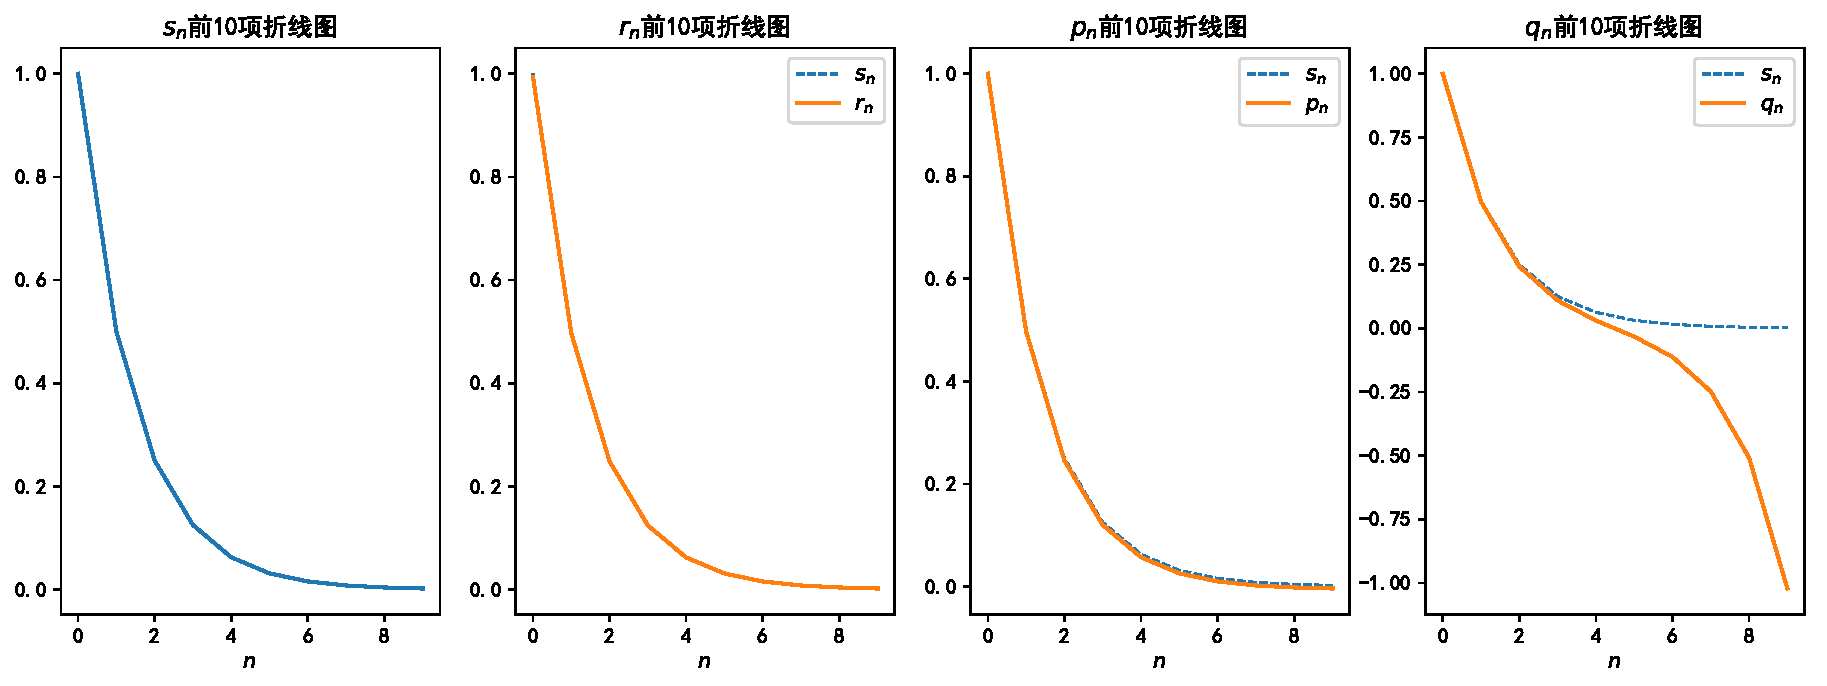
\includegraphics[width=\linewidth]{fig1.pdf}
\end{figure}

数列$\{s_n\}$与$\{r_n\}$,$\{p_n\}$,$\{q_n\}$之差的前10项:

\begin{table}[H]
	\centering
	\caption{生成序列误差表}
	\begin{tabular}{clll}
		\hline
		$n$ & \multicolumn{1}{c}{$s_n - r_n$} & \multicolumn{1}{c}{$s_n - p_n$} & \multicolumn{1}{c}{$s_n - q_n$} \\ \hline
		1   & 0.006000000000            & 0.000000000000            & 0.000000000000            \\
		2   & 0.003000000000            & 0.003000000000            & 0.003000000000            \\
		3   & 0.001500000000            & 0.004500000000            & 0.007500000000            \\
		4   & 0.000750000000            & 0.005250000000            & 0.015750000000            \\
		5   & 0.000375000000            & 0.005625000000            & 0.031875000000            \\
		6   & 0.000187500000            & 0.005812500000            & 0.063937500000            \\
		7   & 0.000093750000            & 0.005906250000            & 0.127968750000            \\
		8   & 0.000046875000            & 0.005953125000            & 0.255984375000            \\
		9   & 0.000023437500            & 0.005976562500            & 0.511992187500            \\
		10  & 0.000011718750            & 0.005988281250            & 1.023996093750            \\ \hline
	\end{tabular}
\end{table}

绘制每个序列的误差变化折线图,

\begin{figure}[H]
	\centering
	\caption{生成序列的误差变化折线图}
	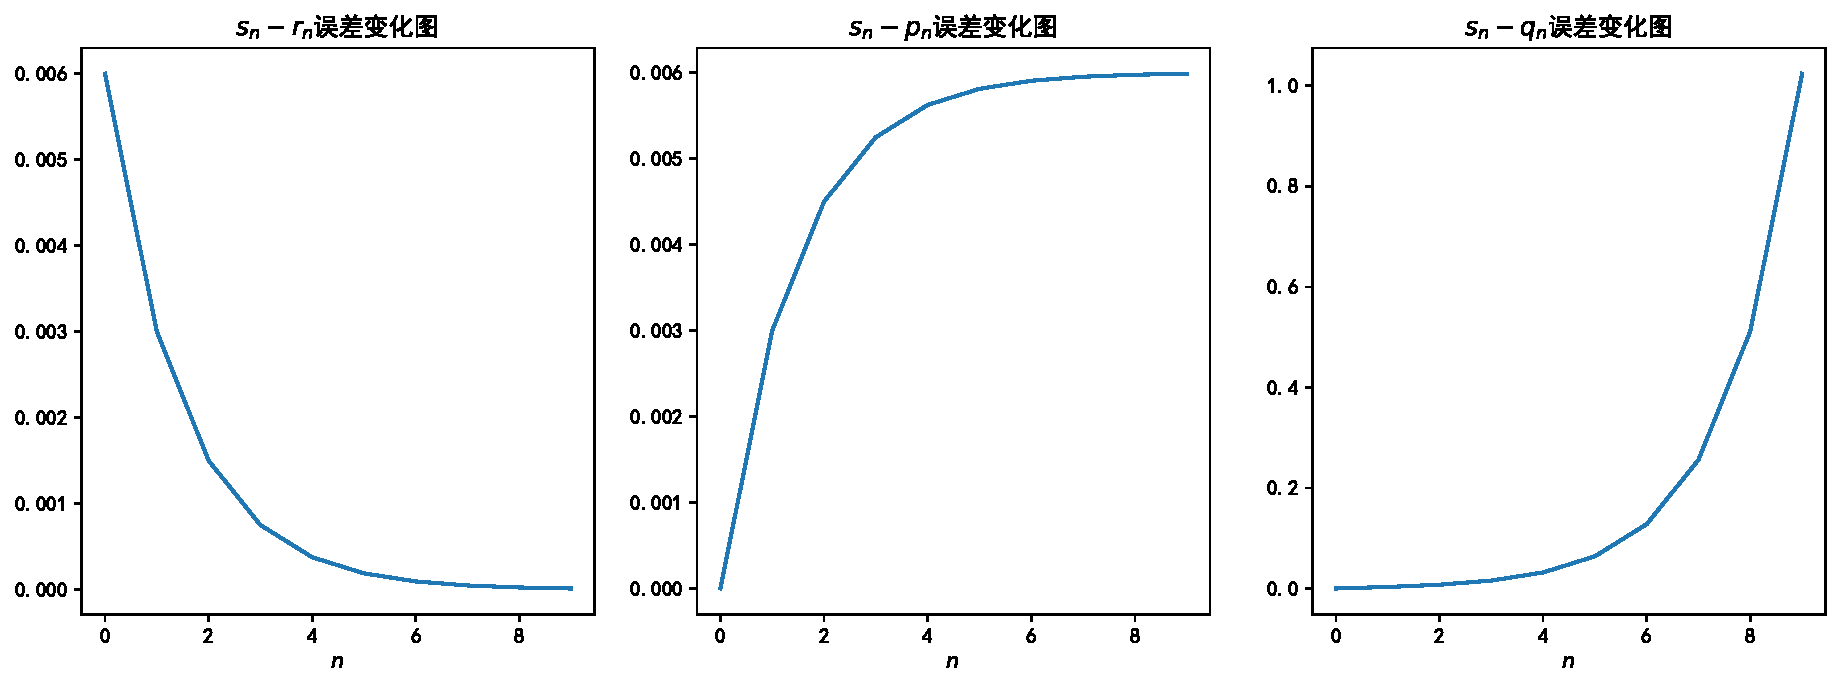
\includegraphics[width=\linewidth]{fig2.pdf}
\end{figure}

将其放在同一坐标系下,

\begin{figure}[H]
	\centering
	\caption{同一坐标系对比图}
	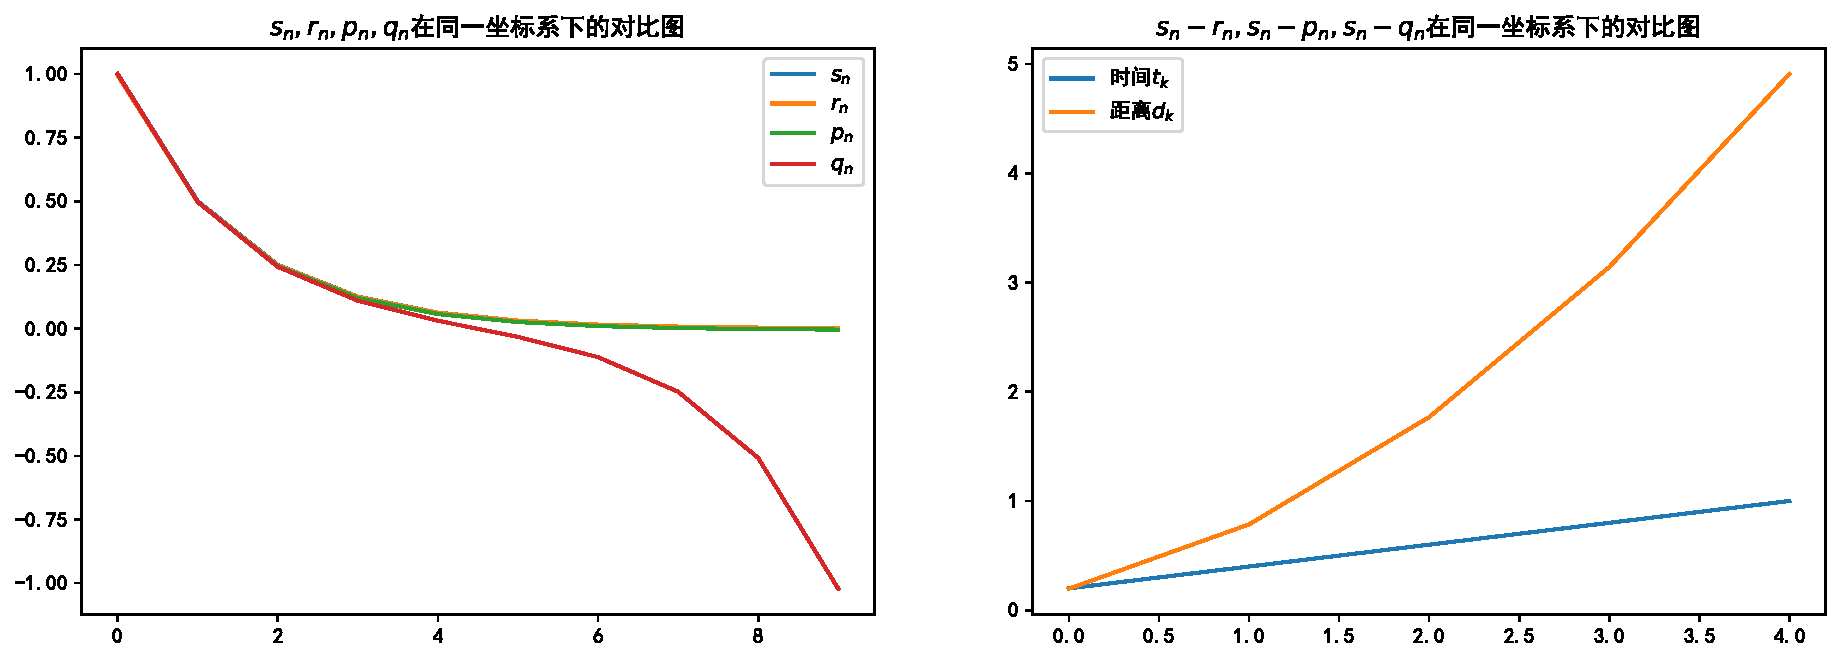
\includegraphics[width=\linewidth]{fig3.pdf}
\end{figure}

\paragraph{分析}
由图表可以发现$p_n$和$r_n$都可以较好地生成需要的序列,而$q_n$却随着$n$的增加离需要构造的序列真实值越来越远。

\section{第2章}


\subsection{题目1}

求方程$2x^2+x-15=0$的正根($x^*=2.5$)近似值,分别用如下三种格式编程计算:

\begin{itemize}
	\item $x_{k+1}=15-x_k^2,k=0,1,2,\cdots$取初始值$x_0=2$
	\item $x_{k+1}=\frac{15}{2x_k+1},k=0,1,2,\cdots$取初始值$x_0=2$
	\item $x_{k+1}=x_k-\frac{2x_k^2+x_k-15}{4x_k+1},k=0,1,2,\cdots$取初始值$x_0=2$
\end{itemize}

依次计算$x_1,x_2,\cdots,x_k,\cdots,$并作图观察解的稳定性、收敛性并分析其原因

\paragraph{不动点法}

设含有n个未知数与n个方程的非线性方程组为F(x)=0,然后把方程组改为便于迭代的等价形式$x=\phi (x)$,由此就可以构造出不动点迭代法的迭代公式为$x_k+1=\phi (x_k)$,如果得到的序列$\{x_k\}$满足$\lim\limits_{k\to \infty} x_k = x^*$,则$x^*$就是$\phi$的不动点,这样就可以求出非线性方程组的解

\paragraph{求解}

直接使用Python对于题目中的三种表达进行计算。

首先,我们对\[x_{k+1}=15-x_k^2,k=0,1,2,\cdots 取初始值x_0=2 \]进行计算。

前四次的迭代结果依次为:\[
x_1=11 \]\[ x_2=-106 \]\[ x_3=-11221 \]\[ x_4=-125910826
\]将前4次的结果作成图像进行观察:
\begin{figure}[H]
	\centering
	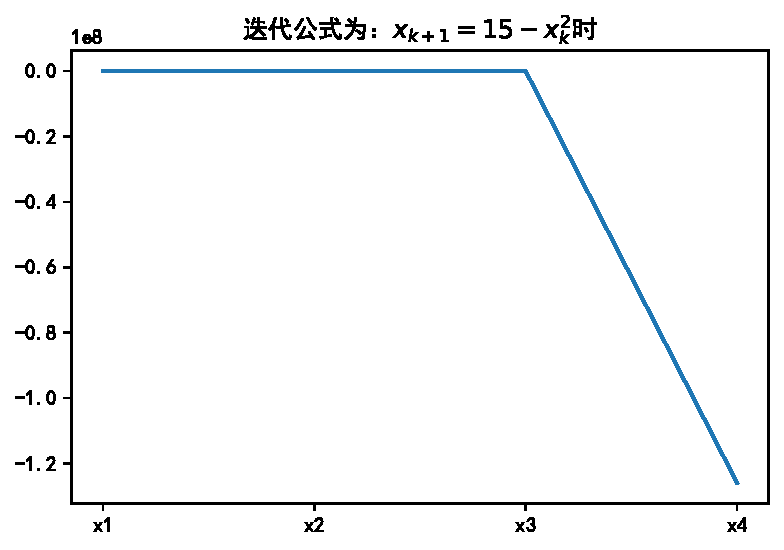
\includegraphics[width=0.7\linewidth]{2-1-1.pdf}
	\caption{}
	\label{fig:2-1-1}
\end{figure}

\paragraph{分析}

由该结果可知,当原方程转换为$x_{k+1}=15-x_k^2,k=0,1,2,\cdots$取初始值$x_0=2$时,方程的解发散,即此时无法求出方程的解。\\



我们对\[ x_{k+1}=\frac{15}{2x_k+1},k=0,1,2,\cdots 取初始值x_0=2 \]进行计算。

前50次的迭代结果依次为:\[ x_1=3.0 \]
\[ x_2=2.142857142857143 \]
\[ x_3=2.8378378378378377 \]
\[ x_4=2.2469635627530367 \]
\[ x_5=2.7302873986735445 \]
\[ x_6=2.3217748374586518 \]
\[ x_7=2.6579016512723084 \]
\[ x_8=2.374994799783671  \]
\[ x_9=2.6087003707152228 \]
\[ x_{10}=2.4125837506412577 \]
\[ \cdots  \]
\[ x_{50}=2.4999395640135855 \]
将前50次的结果作成图像进行观察:
\begin{figure}[H]
	\centering
	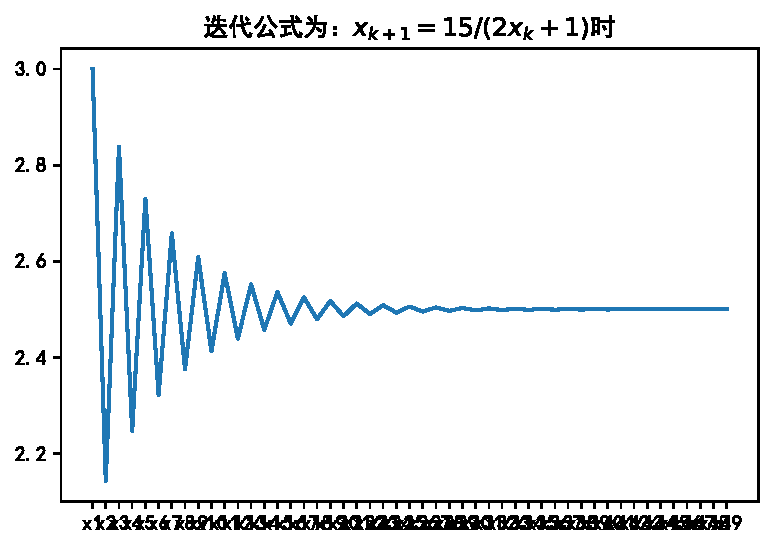
\includegraphics[width=0.7\linewidth]{2-1-2.pdf}
	\caption{}
	\label{fig:2-1-2}
\end{figure}

\paragraph{分析}

由该结果可知,当原方程转换为$x_{k+1}=\frac{15}{2x_k+1},k=0,1,2,\cdots$取初始值$x_0=2$时,方程的解收敛到了2.50,证明该式使用不动点迭代可以得到方程的解。\\


我们对\[ x_{k+1}=x_k-\frac{2x_k^2+x_k-15}{4x_k+1},k=0,1,2,\cdots 取初始值x_0=2 \]进行计算。

前6次的迭代结果依次为:\[ x_{1}=2.5555555555555554 \]
\[ x_{2}=2.5005500550055006 \]
\[ x_{3}=2.5000000550000006 \]
\[ x_{4}=2.5000000000000004 \]
\[ x_{5}=2.5 \]
\[ x_{6}=2.5 \]
将前10次的结果作成图像进行观察:
\begin{figure}[H]
	\centering
	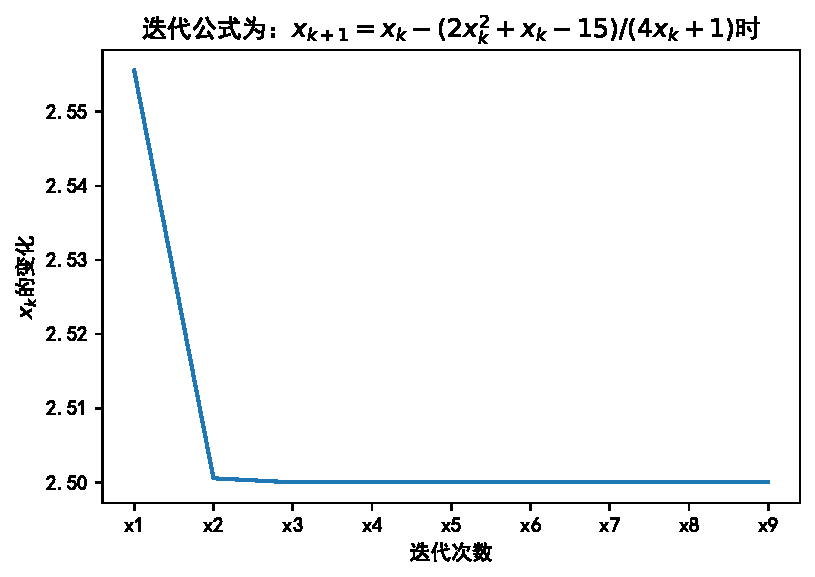
\includegraphics[width=0.7\linewidth]{2-1-3.pdf}
	\caption{}
	\label{fig:2-1-2}
\end{figure}

\paragraph{分析}

由该结果可知,当原方程转换为$x_{k+1}=x_k-\frac{2x_k^2+x_k-15}{4x_k+1},k=0,1,2,\cdots$取初始值$x_0=2$时,方程的解收敛到了2.50,证明该式使用不动点迭代可以得到方程的解。

\subsection{题目2}

证明方程\[2-3x-sin(x)=0\]在$(0,1)$内有且只有一个实根,使用二分法求误差不大于0.0005的根,及其需要的迭代次数。


\paragraph{证明}
~\\
$f(x)=2-3x-sin(x)$\\对f(x)求导,得$f'(x)=-3-cos(x)$\\当$x \in (0,1)$时,$f'(x)<0$,即$f(x)$在(0,1)单调递减\\又,$f(1)=-1-sin(1)<0,f(0)=2>0$\\故可知在(0,1)内,方程在有且只有一个实根


\paragraph{二分法}
~\\
如果$f\in C(a,b)$,且存在数$r\in[a,b]$,满足$f(r)=0$。如果$f(a)f(b)<0$则在区间$[a,b]$内有奇数个零点,若只有一个零点,可以递归用下述方法找到零点:

每次取中点z,若$f(z)=0$,则z就是零点。如果$f(z)f(a)<0$则区间变换到$[a,z]$,否则区间变为$[z,b]$。

从上述递归中容易知道,每次都将零点存在的区间缩小一倍,所以如果在区间$[a,b]$上,如果迭代$n$次,可以得到精度为:
$(b-a)/2^{n+1} $

因此,当$n\rightarrow \infty $的时候,上式右边趋于0,所以得到$r→c_n$,所以只要$n$足够大, 最后一定会收敛到目标点。


\paragraph{求解}

使用二分法进行求解得到根,经过计算,10次迭代后,解收敛,得到解0.505371094。

随迭代次数,解和误差的变化如下表:
\begin{table}[H]
	\centering
	\caption{二分法迭代解和误差的变化}
	\begin{tabular}{lll}
		\hline
		迭代次数 & $x_{mid}$          & 误差                   \\ \hline
		0  & 0.5         & 0.020574461             \\
		1  & 0.75        & -0.93163876             \\
		2  & 0.625       & -0.460097273            \\
		3  & 0.5625      & -0.220802674            \\
		4  & 0.53125     & -0.100361455            \\
		5  & 0.515625    & -0.039953686            \\
		6  & 0.5078125   & -0.009704452            \\
		7  & 0.50390625  & 0.005431321             \\
		8  & 0.505859375 & -0.00213749             \\
		9  & 0.504882813 & 0.001646685             \\
		10 & 0.505371094 & -0.0002454600314260591 \\ \hline
	\end{tabular}
\end{table}

\begin{figure}[H]
	\centering
	\caption{二分法求解过程图}
	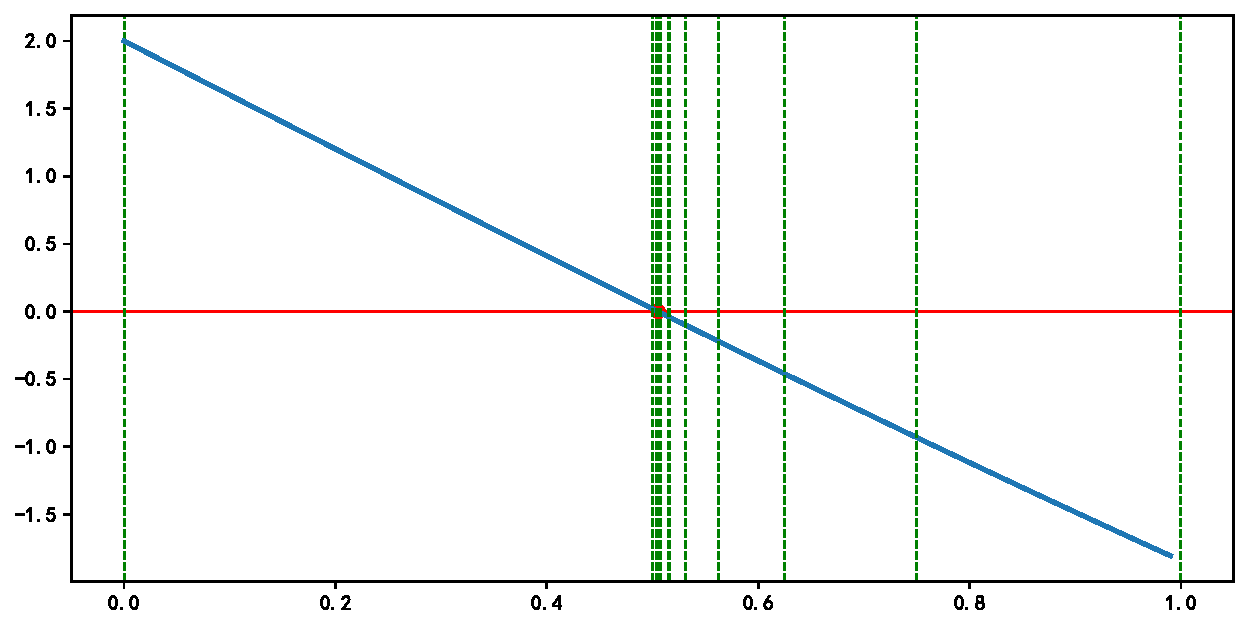
\includegraphics[width=\linewidth]{2-2-1.pdf}
\end{figure}

\paragraph{代码}
~\\
\begin{minted}{python}
def bisection(f, a, b, max_iter, ax=None, px=None):
    if ax is not None:
        ax.axhline(y=0, color='red', linestyle='-', linewidth=1)
        ax.axvline(x=a, linestyle='--', c='green', linewidth=1)
        ax.axvline(x=b, linestyle='--', c='green', linewidth=1)
        ax.plot(px, f(px), linewidth=2)
    if f(a) * f(b) >= 0:
        print("二分法失败.")
        return None
    for _ in range(max_iter):
        c = (a + b) / 2
        if ax is not None:
            ax.axvline(x=c, linestyle='--', c='green', linewidth=1)
        fc = f(c)
        if f(a) * fc < 0:
            b = c
        elif f(b) * fc < 0:
            a = c
        elif fc == 0:
            print("找到准确的解.")
            return c
        else:
            print("二分法失败.")
            return None
    if ax is not None:
        ax.scatter((a + b) / 2, 0, c='red')
    return (a + b) / 2
\end{minted}

\begin{minted}{python}
x = sp.Symbol('x')
f = 2 - 3*x-sp.sin(x)
df = sp.diff(f)
f_eval = sp.lambdify(x, f)
df_eval = sp.lambdify(x, df)
display(Math('f(x) = %s 的导函数为 f^\prime(x) = %s.' % (sp.latex(f), sp.latex(df))))
fig, ax = plt.subplots(nrows=1, ncols=1, figsize=(10, 5))
px = np.arange(0, 1, 0.01)
bisection(f_eval, 0, 1, 10, ax, px)
plt.savefig('2-2-1.pdf', bbox_inches='tight')
\end{minted}


\subsection{题目3}

利用牛顿法求解方程
$$\frac{1}{2}+\frac{1}{4}x^2-x\sin x-\frac{1}{2}\cos2x=0$$
分别取$x_0=\frac{\pi}{2},5\pi,10\pi$,使精度不超过$10^{-5}$,比较初值对计算结果的影响。

\paragraph{牛顿法}
~\\
推导:假设$f\in C^2\left[a,b\right]$, 并且$x^{*}$是$f\left(x \right) = 0$的一个解.

令$\overline{x} \in \left[a,b\right]$是对$x_{*}$的一个近似, 使得$f'\left(\overline{x} \right) \neq 0$且$\left|\overline{x} - x^{*} \right|$比较小. 考虑$f\left(x\right)$在$\overline{x}$处展开的一阶泰勒多项式$f\left(x\right) = f\left(\overline{x} \right) + \left(x - \overline{x}\right) f' \left(\overline{x} \right) + \frac{\left(x-\overline{x}\right)^2}{2}f^{''}\left(\xi \left(x\right) \right)$, 其中$\xi \left(x \right)$在$x$和$\overline{x}$之间. 因为$f\left(x^{*}\right)=0$, 令$x=x^{*}$, 此时有
$0 = f\left(x^{*}\right) = f\left(\overline{x} \right) + \left(x^{*} - \overline{x}\right) f' \left(\overline{x} \right) + \frac{\left(x^{*}-\overline{x}\right)^2}{2}f^{''}\left(\xi \left(x\right) \right)$. 忽略余项, 得到
$0 = f\left(x^{*}\right) \approx f\left(\overline{x} \right) + \left(x^{*} - \overline{x}\right) f' \left(\overline{x} \right)$

求得$$x^{*} \approx \overline{x} - \frac{f\left(\overline{x}\right)}{f'\left(\overline{x}\right)}$$

因此定义迭代序列为:
$x_n = x_{n-1} - \frac{f\left(x_{n-1} \right)}{f'\left(x_{n-1} \right)},\forall n \geq 1$.

\paragraph{求解}
~\\
使用Python的\texttt{sympy包}求得$f(x) = \frac{x^{2}}{4} - x \sin{\left (x \right )} - \frac{1}{2} \cos{\left (2 x \right )} + \frac{1}{2}$ 的导函数为 $$f^\prime(x) = - x \cos{\left (x \right )} + \frac{x}{2} - \sin{\left (x \right )} + \sin{\left (2 x \right )}$$

然后我们做出$f(x) = \frac{x^{2}}{4} - x \sin{\left (x \right )} - \frac{1}{2} \cos{\left (2 x \right )} + \frac{1}{2}$及其导函数的图像进行观察。

\begin{figure}[H]
	\centering
	\caption{$f(x) = \frac{x^{2}}{4} - x \sin{\left (x \right )} - \frac{1}{2} \cos{\left (2 x \right )} + \frac{1}{2}$及其导函数图像}
	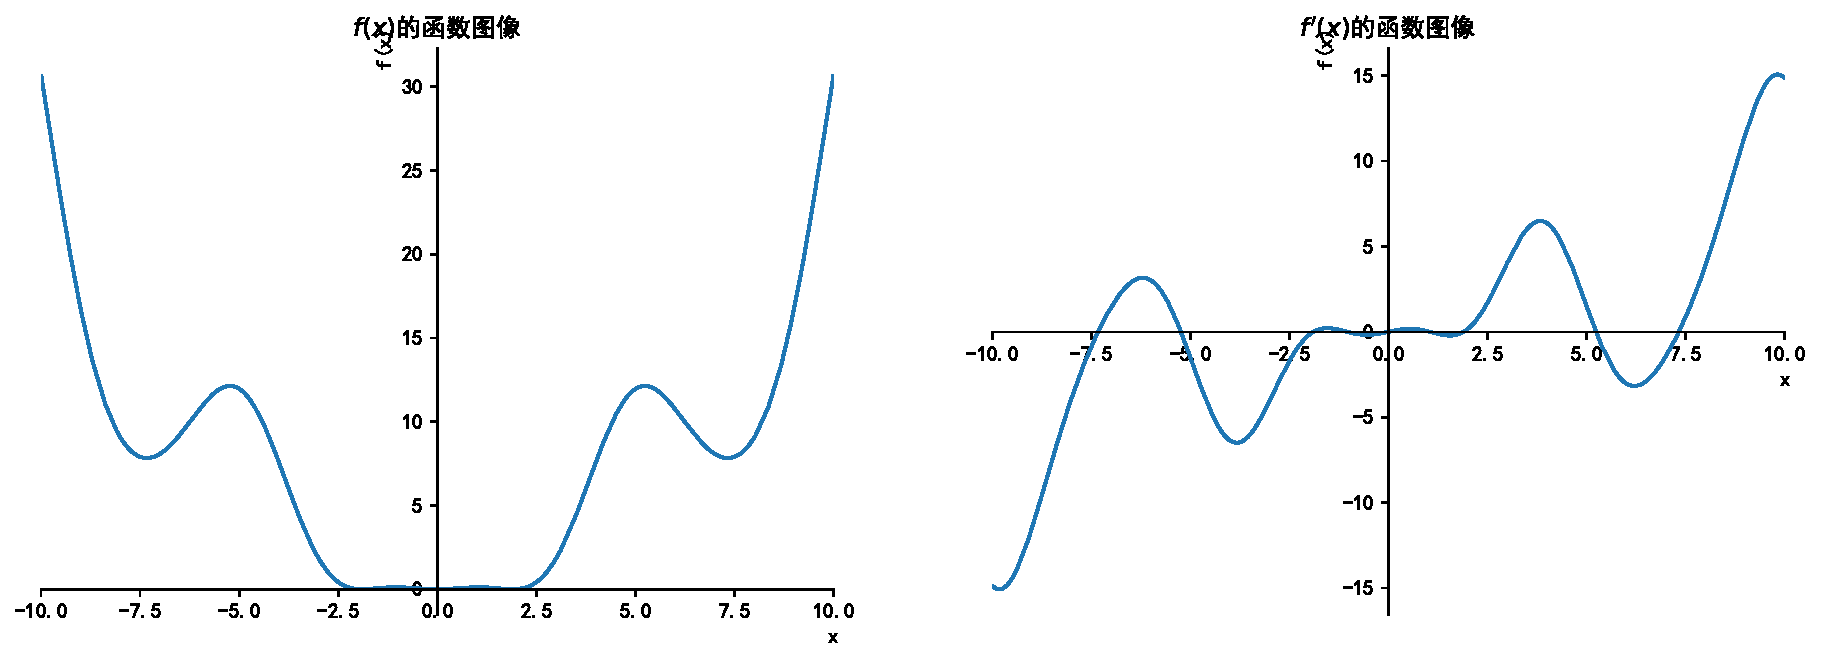
\includegraphics[width=\linewidth]{fig4.pdf}
\end{figure}


观察图像可知,函数零点在$(-2, 2)$这段区间上,因此我们将其放大进行观察:

\begin{figure}[H]
	\centering
	\caption{$f(x)$在$(-2, 2)$区间上的放大图}
	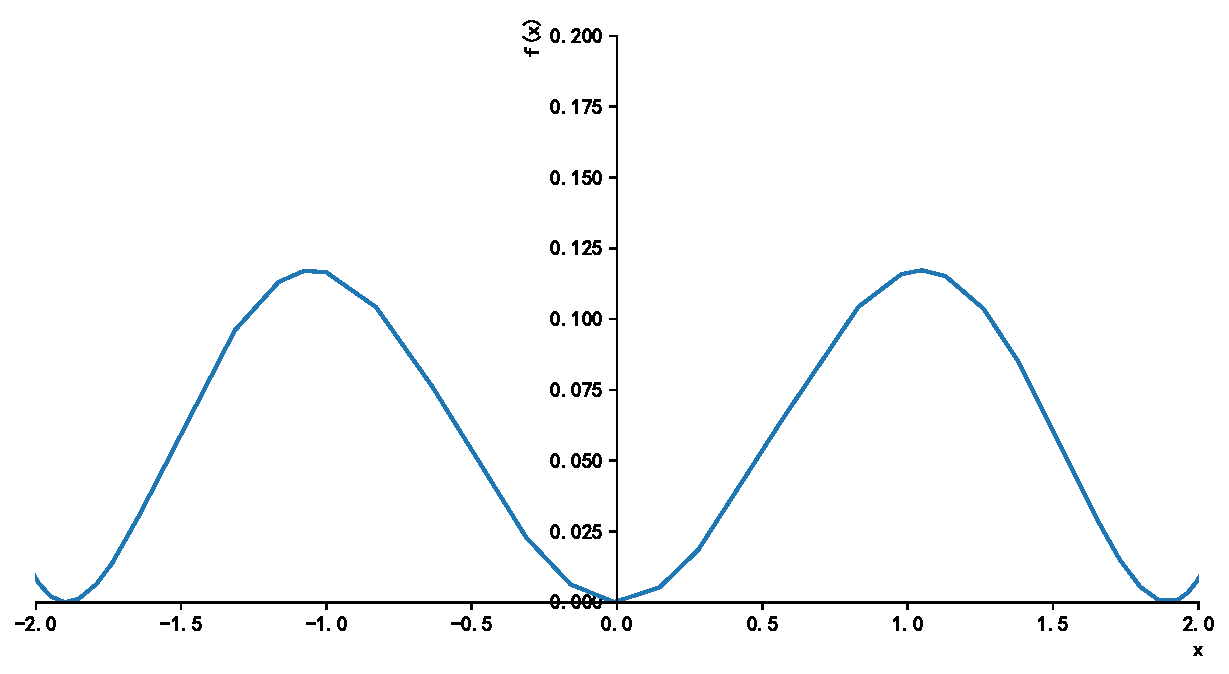
\includegraphics[width=\linewidth]{fig5.pdf}
\end{figure}

然后使用牛顿法求解方程,分别取$x_0=\frac{\pi}{2},5\pi,10\pi$。

\paragraph{$x_0=\frac{\pi}{2}$时} 在6次迭代后找到零点\[x = 1.8924896245342444\]

\begin{figure}[H]
	\centering
	\caption{$x_0 = \pi / 2$ 时牛顿法的过程图}
	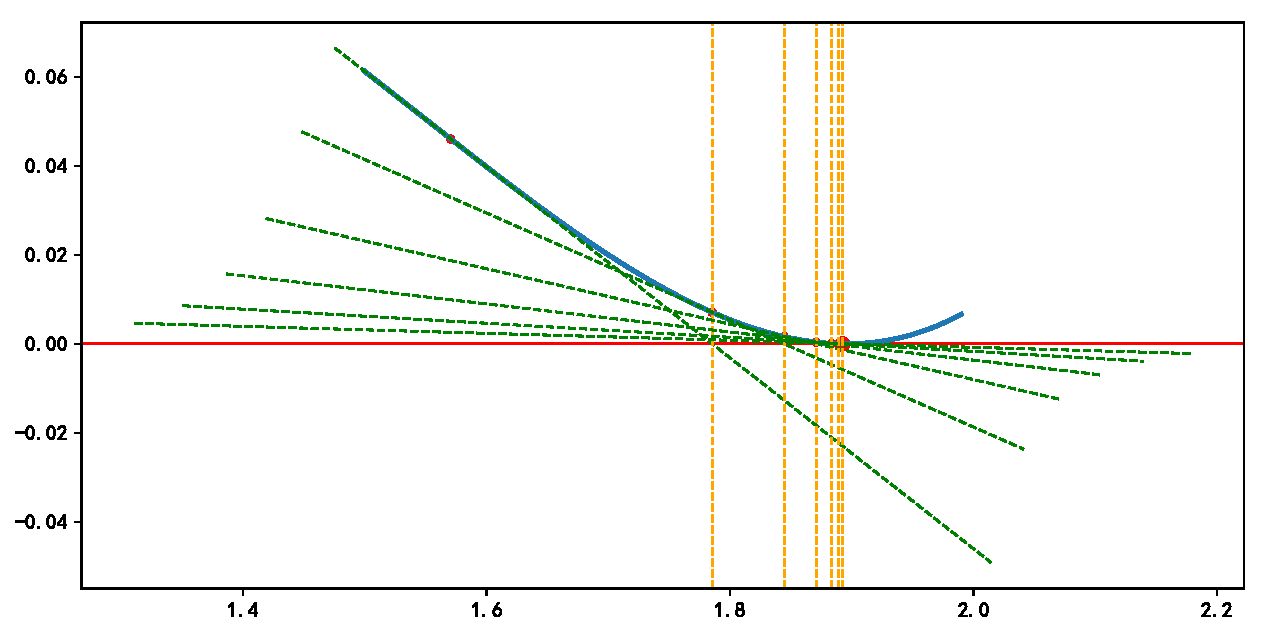
\includegraphics[width=\linewidth]{fig6.pdf}
\end{figure}

\paragraph{$x_0=5\pi$时} 在10次迭代后找到零点\[x = 1.8927898018266247\]

\begin{figure}[H]
	\centering
	\caption{$x_0 = 5\pi$ 时牛顿法的过程图}
	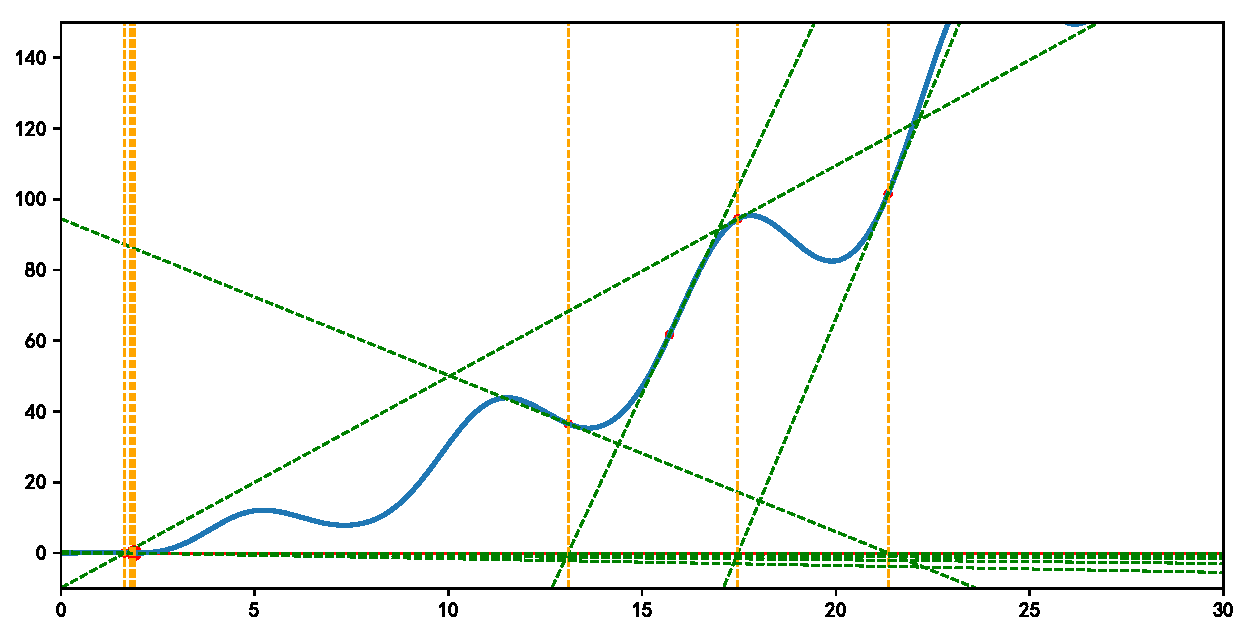
\includegraphics[width=\linewidth]{fig7.pdf}
\end{figure}

\paragraph{$x_0=10\pi$时} 在10313次迭代后找到零点\[x = 1.898094316843809\]

由于当$x_0=10\pi$时时迭代次数过多,计算量过大,所以难以将计算过程进行可视化,仅计算其结果,不进行可视化。

\paragraph{代码}
~\\
\begin{minted}{python}
def newton(f, df, x0, eps, max_iter, ax=None, px=None):
    x = x0
    if ax is not None:
        ax.axhline(y=0, color='red', linestyle='-', linewidth=1)
        ax.plot(px, f(px), linewidth=2)
\end{minted}
\begin{minted}{python}
    for n in range(max_iter):
        fx = f(x)
        if ax is not None:
            ax.scatter(x, fx, c='red', marker='.')
        if abs(fx) < eps:
            print('在%d次迭代后找到解.' % n)
            if ax is not None:
                ax.scatter(x, fx, c='red')
            return x
        dfx = df(x)
        if ax is not None:
            abline(ax, x, fx, dfx)
        if dfx == 0:
            print('导数值为0,无法找到解.')
            return None
        x = x - fx / dfx
        if ax is not None:
            ax.axvline(x=x, linestyle='--', c='orange', 
                       linewidth=1)
    print('超过最大迭代次数,无法找到解.')
    return None
    
px = np.arange(1.5, 2.0, 0.01)
display(Math('找到零点x = %s.' % 
  newton(f_eval, df_eval, np.pi / 2, 1e-5, 100, ax, px)))
px = np.arange(0, 30, 0.1)
plt.xlim(0, 30)
plt.ylim(-10, 150)
display(Math('找到零点x = %s.' %
  newton(f_eval, df_eval, 5 * np.pi, 1e-5, 100, ax, px)))
display(Math('找到零点x = %s.' %
  newton(f_eval, df_eval, 10 * np.pi, 1e-5, 20000)))
\end{minted}

\paragraph{解与迭代次数的关系探究}
~\\
下面对解和迭代次数的关系进行探究(以初值$x_0 = \frac{\pi}{2}$为例):

\begin{figure}[H]
	\centering
	\caption{解与迭代次数的关系图}
	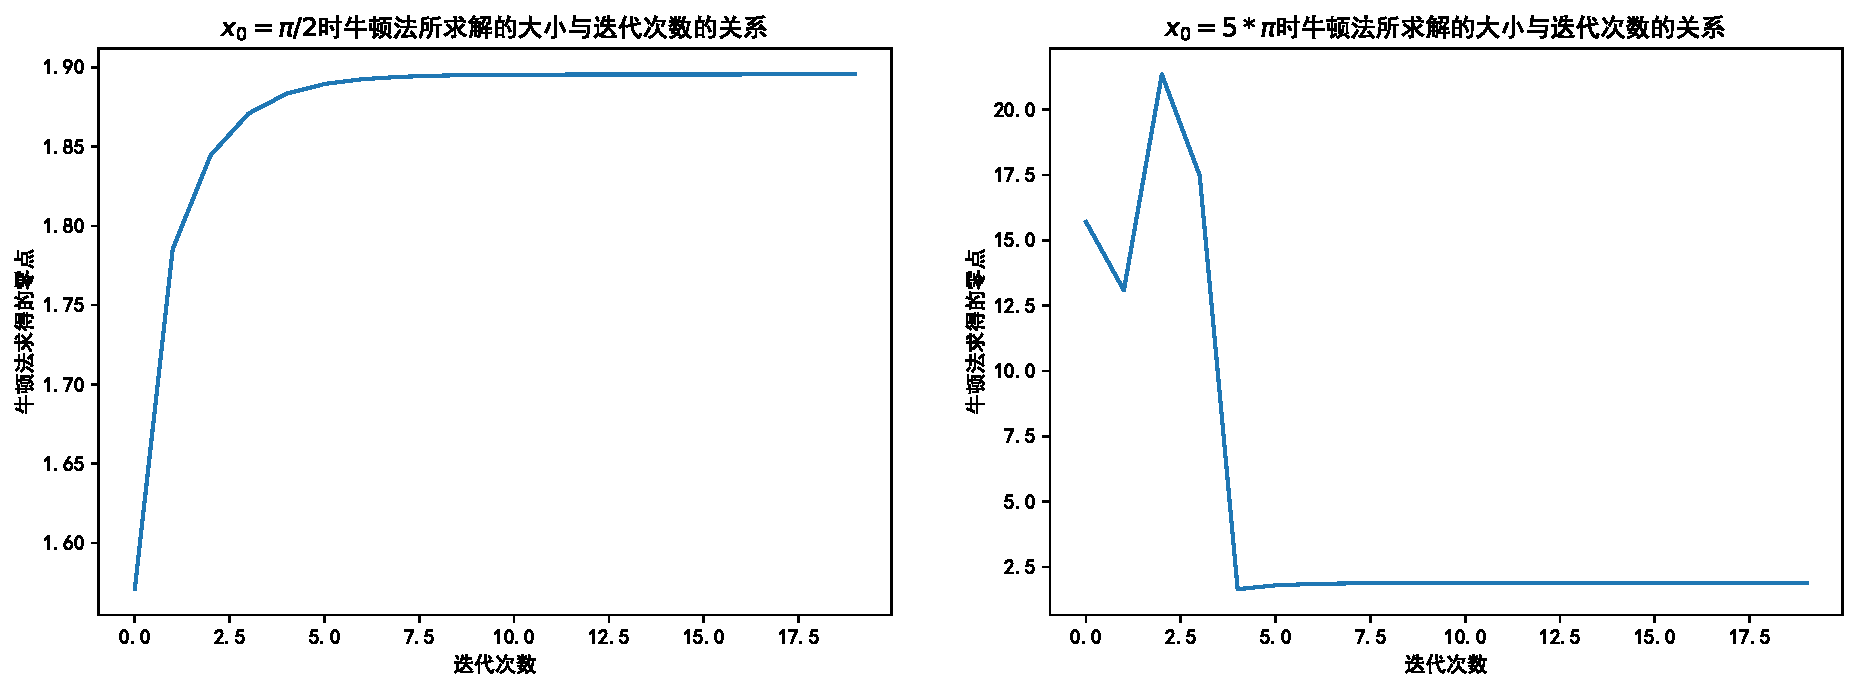
\includegraphics[width=\linewidth]{fig8.pdf}
\end{figure}

随着迭代次数的增加,解的大小的绝对量变化越来越小;初值的选择对于迭代的次数与解的质量有很大关系。

\subsection{题目4}

已知$$f\left(x\right) = 5x - e^x$$
在$\left(0,1\right)$之间有一个实根,试分别用二分法、牛顿法、割线法、错位法设计相应的计算格式,并编程求解。

\paragraph{二分法}
~\\
如果$f\in C(a,b)$,且存在数$r\in[a,b]$,满足$f(r)=0$。如果$f(a)f(b)<0$则在区间$[a,b]$内有奇数个零点,若只有一个零点,可以递归用下述方法找到零点:

每次取中点z,若$f(z)=0$,则z就是零点。如果$f(z)f(a)<0$则区间变换到$[a,z]$,否则区间变为$[z,b]$。

从上述递归中容易知道,每次都将零点存在的区间缩小一倍,所以如果在区间$[a,b]$上,如果迭代$n$次,可以得到精度为:
$(b-a)/2^{n+1} $

因此,当$n\rightarrow \infty $的时候,上式右边趋于0,所以得到$r→c_n$,所以只要$n$足够大, 最后一定会收敛到目标点。

\paragraph{求解}
~\\
使用二分法进行求解得到根$0.25917110181907377$

\begin{figure}[H]
	\centering
	\caption{二分法求解过程图}
	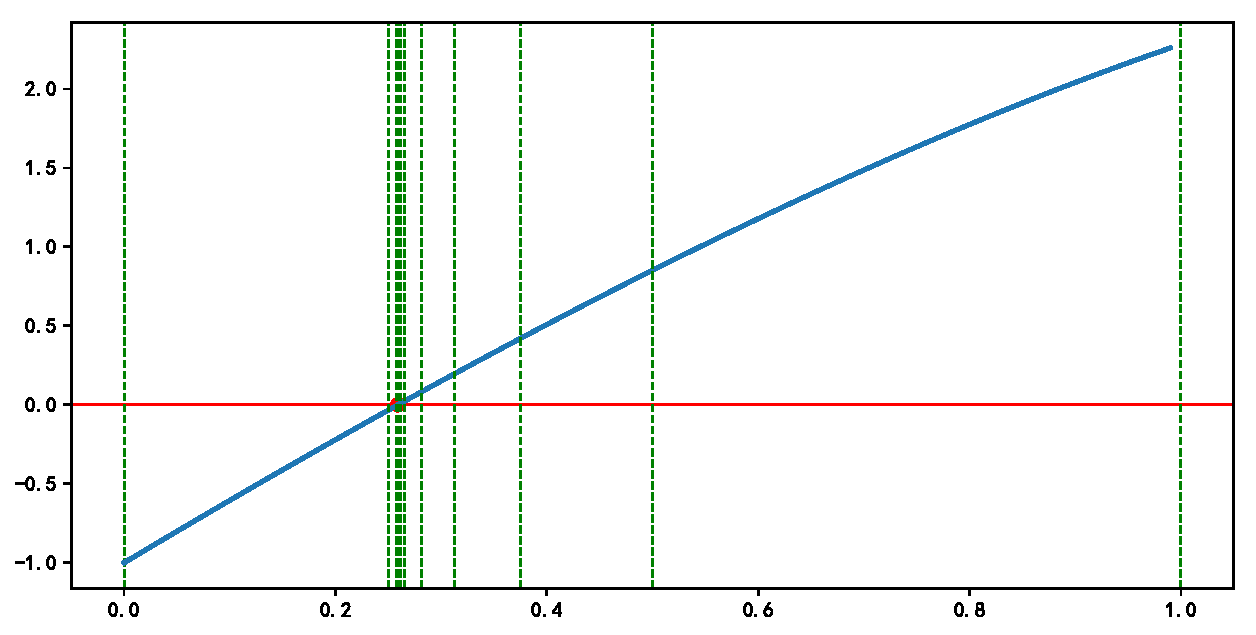
\includegraphics[width=\linewidth]{fig9.pdf}
\end{figure}

\paragraph{二分法代码}
~\\
\begin{minted}{python}
def bisection(f, a, b, max_iter, ax=None, px=None):
    if ax is not None:
        ax.axhline(y=0, color='red', linestyle='-', linewidth=1)
        ax.axvline(x=a, linestyle='--', c='green', linewidth=1)
        ax.axvline(x=b, linestyle='--', c='green', linewidth=1)
        ax.plot(px, f(px), linewidth=2)
    if f(a) * f(b) >= 0:
        print("二分法失败.")
        return None
    for _ in range(max_iter):
        c = (a + b) / 2
        if ax is not None:
            ax.axvline(x=c, linestyle='--', c='green', linewidth=1)
\end{minted}
\begin{minted}{python}
        fc = f(c)
        if f(a) * fc < 0:
            b = c
        elif f(b) * fc < 0:
            a = c
        elif fc == 0:
            print("找到准确的解.")
            return c
        else:
            print("二分法失败.")
            return None
    if ax is not None:
        ax.scatter((a + b) / 2, 0, c='red')
    return (a + b) / 2
\end{minted}

\paragraph{牛顿法}
~\\
首先使用Python的\texttt{sympy}包对函数$f\left(x\right) = 5x - e^x$进行求导,得$f(x) = 5 x - e^{x}$的导函数为$ f^\prime(x) = - e^{x} + 5$,然后对其图像进行观察。

\begin{figure}[H]
	\centering
	\caption{$f(x)$与$f^\prime(x)$的函数图像}
	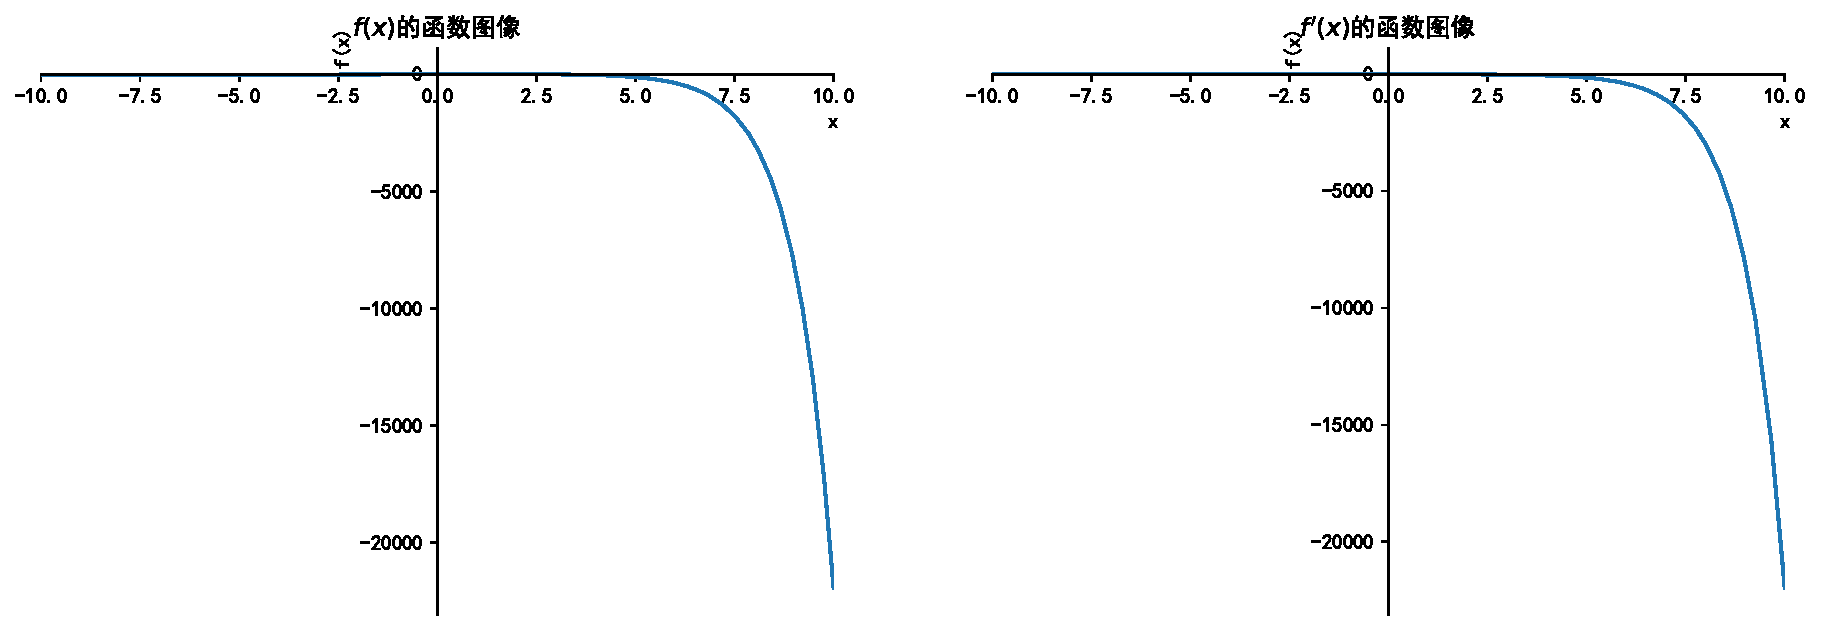
\includegraphics[width=.9\linewidth]{fig_1.pdf}
\end{figure}

运行牛顿法在4次迭代后找到解$0.2591711017819102$。

\begin{figure}[H]
	\centering
	\caption{牛顿法过程图}
	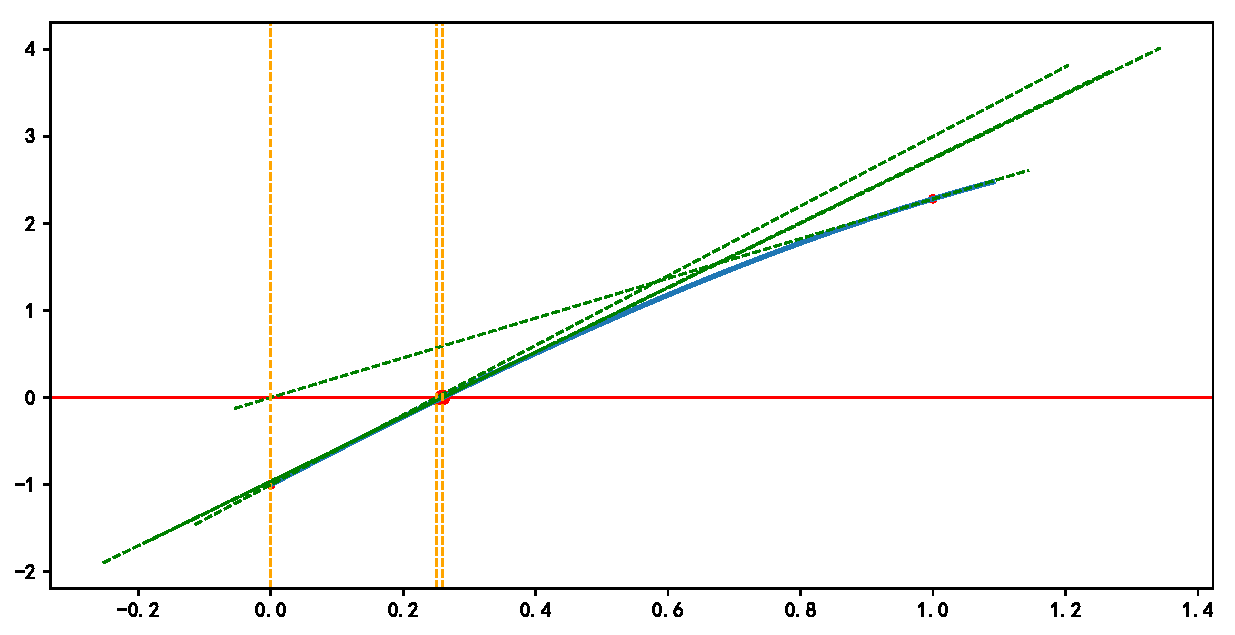
\includegraphics[width=.87\linewidth]{fig10.pdf}
\end{figure}

\paragraph{牛顿法代码}

牛顿法代码请见题目1。

\begin{minted}{python}
px = np.arange(0, 1.1, 0.01)
newton(f_eval, df_eval, 1, 1e-5, 100, ax, px)
\end{minted}
 
\paragraph{割线法}
~\\
推导: 用割线近似代替牛顿法中的切线.

得到公式$x_{k+1} = x_k - f\left(x_k\right) \frac{x_k - x_{k-1}}{f\left(x_k\right) - f\left( x_{k-1}\right)}$。

运行割线法找到解$0.25917110181907377$。

\begin{figure}[H]
	\centering
	\caption{割线法过程图}
	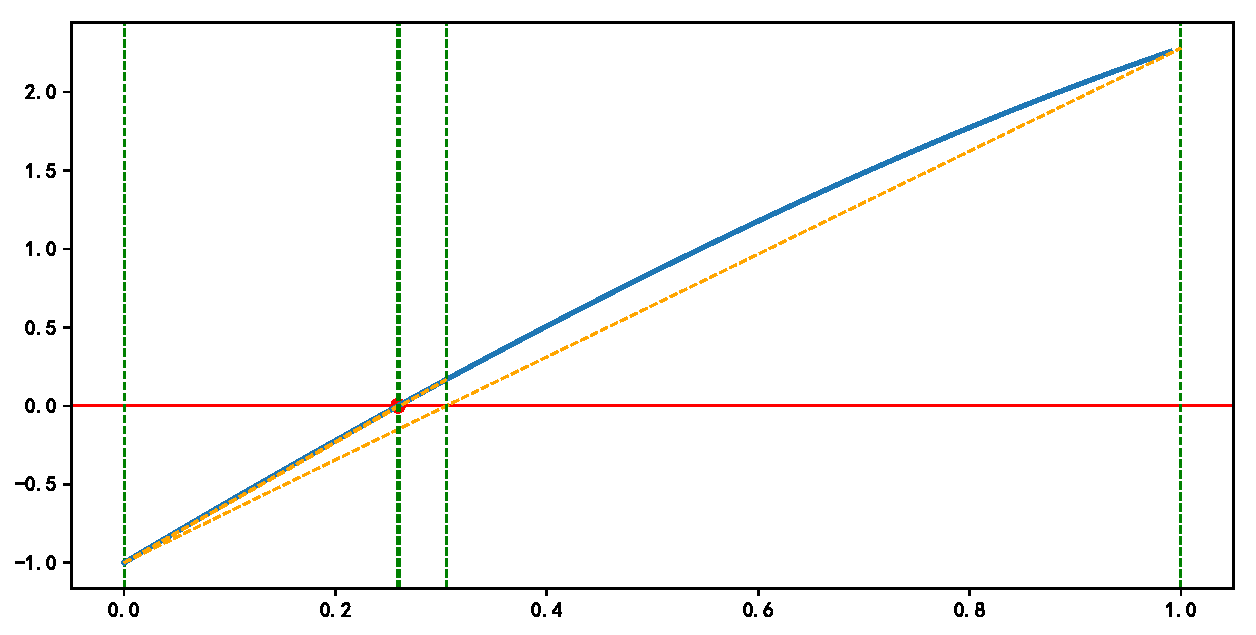
\includegraphics[width=.87\linewidth]{fig11.pdf}
\end{figure}

\paragraph{割线法代码}
~\\
\begin{minted}{python}
def secant(f, a, b, max_iter, ax=None, px=None):
    if ax is not None:
        ax.axhline(y=0, color='red', linestyle='-', linewidth=1)
        ax.axvline(x=a, linestyle='--', c='green', linewidth=1)
        ax.axvline(x=b, linestyle='--', c='green', linewidth=1)
        ax.plot(px, f(px), linewidth=2)
    if f(a) * f(b) >= 0:
        print("割线法失败.")
        return None
    for _ in range(max_iter):
        fa, fb = f(a), f(b)
        c = a - fa * (b - a) / (fb - fa)
        if ax is not None:
            ax.plot([a, b], [fa, fb], c='orange', linestyle='--', 
                    linewidth=1)
            ax.axvline(x=c, linestyle='--', c='green', linewidth=1)
        fc = f(c)
        if fa * fc < 0:
            b = c
        elif fb * fc < 0:
            a = c
        elif fc == 0:
            print("找到准确的解.")
            return c
        else:
            print("割线法失败.")
            return None
    if ax is not None:
        ax.scatter(a - f(a) * (b - a) / (f(b) - f(a)), 0, c='red')
    return a - f(a) * (b - a) / (f(b) - f(a))
\end{minted}

\paragraph{错位法}
~\\
推导:要在区间$\left[p_0,p_1 \right]$上寻找$f\left(x\right) = 0$的解, 其中$f\left(p_0 \right) f\left(p_1 \right) < 0$.

使用与切线法相同的方式, 找到近似点$p_2$.

为确定使用哪一条线计算$p_3$, 计算$f\left(p_2 \right) f\left(p_1 \right)$和$f\left( p_2\right) f\left(p_0 \right)$.

如果$f\left(p_2 \right) f\left(p_1 \right) < 0$, 说明$p_1,p_2$中间包含了一个根, 那么取$\left(p_1,f\left(p_1\right) \right),\left(p_2,f\left(p_2 \right)\right)$线段的斜率, 作为切线法中的斜率.

运行错位法找到解$0.25917110181907377$。

\begin{figure}[H]
	\centering
	\caption{错位法过程图}
	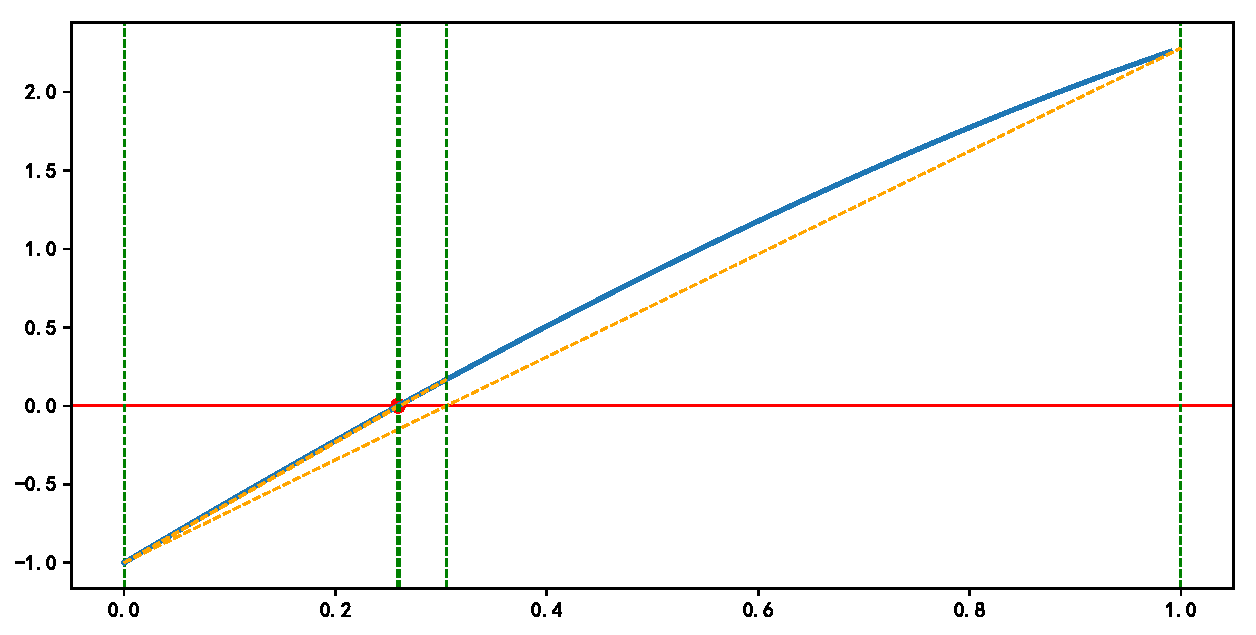
\includegraphics[width=\linewidth]{fig12.pdf}
\end{figure}

\paragraph{错位法代码}
~\\
\begin{minted}{python}
def secant(f, a, b, max_iter, ax=None, px=None):
    if ax is not None:
        ax.axhline(y=0, color='red', linestyle='-', linewidth=1)
        ax.axvline(x=a, linestyle='--', c='green', linewidth=1)
        ax.axvline(x=b, linestyle='--', c='green', linewidth=1)
        ax.plot(px, f(px), linewidth=2)
    if f(a) * f(b) >= 0:
        print("割线法失败.")
        return None
\end{minted}
\begin{minted}{python}
    for _ in range(max_iter):
        fa, fb = f(a), f(b)
        c = a - fa * (b - a) / (fb - fa)
        if ax is not None:
            ax.plot([a, b], [fa, fb], c='orange', linestyle='--', 
                    linewidth=1)
            ax.axvline(x=c, linestyle='--', c='green', linewidth=1)
        fc = f(c)
        if fa * fc < 0:
            b = c
        elif fb * fc < 0:
            a = c
        elif fc == 0:
            print("找到准确的解.")
            return c
        else:
            print("割线法失败.")
            return None
    if ax is not None:
        ax.scatter(a - f(a) * (b - a) / (f(b) - f(a)), 0, c='red')
    return a - f(a) * (b - a) / (f(b) - f(a))

fig, ax = plt.subplots(nrows=1, ncols=1, figsize=(10, 5))
px = np.arange(0, 1, 0.01)
regula(f_eval, 0, 1, 100, ax, px)
\end{minted}
\section{第三章}

\subsection{题目1}

求解线性方程组
\begin{align}
	&4x-y+z=7\\
	&4x-8y+z=-21\\
	&-2x+y+5z=15
\end{align}

\begin{enumerate}
	\item 使用LU分解求此方程组
	\item 分别用Jacobi,Gauss-Seidel方法求解此方程组
\end{enumerate}

\subsubsection{题目1.1}

使用LU分解求此方程组。

\paragraph{LU分解}
~\\
给定一个无行交换的高斯消去法可求解一般线性方程组$AX=B$,则矩阵A可分解为一个下三角矩阵L和一个上三角矩阵U的乘积:
\begin{center}
	$A=LU$ 
\end{center}
而且L的对角线元素为1,U的对角线元素非零。
得到LU矩阵之后,原方程变为:
\begin{center}
	$LUX=B$ 
\end{center}
这时可以先把UX当成新的未知数,即求解
$LX_{new}=B$
得到$X_{new}w$之后,再求解
$UX=X_{new}$
最终得到X.

\paragraph{分解矩阵}
~\\
利用已知求未知。最开始已知L的对角线全是1,所以用L的第一行分别与U的第一列、第二列…第n列相乘,得到U的第一行。然后用L的第二行与U的第一列相乘求得L中第二行的所有元素,然后用L的第二行分别与U的所有列相乘求得U的第二行,然后一直重复这样的步骤,就可以得到分解的LU矩阵。
\paragraph{求解矩阵$X_{new}$}
~\\
用L的第一行乘以$X_{new}$的列,求得$X_{new}$的第一行,然后用L的第二行乘以$X_{new}$的列,求得$X_{new}$的第二行。重复这样的步骤就可以得到$X_{new}$的所有值。
\paragraph{求解矩阵$X$}
~\\
类似$X_{new}$的求法,但是是从U矩阵的最后一行向上分别和X的列相乘。
LU分解的代码和分解之后求解方程组的代码:

设$\mathbf{A} = \left(a_{i,j}\right)_{n \times n}$, 分解为$\mathbf{A} = \mathbf{LU}$的形式, 其中$\mathbf{L}$为对角元为1的下三角矩阵, $\mathbf{U}$为上三角矩阵. 即
$$
\left(
\begin{matrix}
a_{11} & a_{12} & \cdots & a_{1n} \\
a_{21} & a_{22} & \cdots & a_{2n} \\
\vdots & \vdots & \ddots & \vdots \\
a_{n1} & a_{n2} & \cdots & a_{nn} \\
\end{matrix}
\right) =
\left(
\begin{matrix}
1 & 0 & \cdots & 0 \\
l_{21} & 1 & \cdots & 0 \\
\vdots & \vdots & \ddots & \vdots \\
l_{n1} & l_{n2} & \cdots & 1 \\
\end{matrix}
\right) 
\left(
\begin{matrix}
u_{11} & u_{12} & \cdots & u_{1n} \\
0 & u_{22} & \cdots & u_{2n}\\
\vdots & \vdots & \ddots & \vdots \\
0 & 0 & \cdots & u_{nn} \\
\end{matrix}
\right)
$$
按照矩阵乘法规则, 比较系数, 可得
$$
\left\{
\begin{aligned}
u_{1j} &= a_{1j}  &\left(j=1,2,\cdots,n\right) \\
l_{i1} &= \frac{a_{i1}}{u_{11}} &\left(i=2,3,\cdots,n \right)\\
u_{ij} &= a_{ij} - \sum_{k=1}^{i-1}l_{ik}u_{kj} &\left(i=2,\cdots,n,j=i,\cdots,n\right) \\
l_{ij} &= \left(a_{ij} - \sum_{k=1}^{j-1}l_{ik}u_{kj}\right) &\left(j=1,2,\cdots,n,i=j+1,\cdots,n\right)
\end{aligned}
\right.$$

分解之后的矩阵:
$$
\mathbf{L} = 
\left(
\begin{matrix}
1 & 0 & 0 \\
1 &  1 & 0 \\
-0.5 &  -0.0714 & 1
\end{matrix}
\right)
\mathbf{U} = 
\left(
\begin{matrix}
4 & -1 & 1 \\
0 &  -7 & 0 \\
0 &  0 & 5.5
\end{matrix}
\right)
$$
方程的解:
\begin{enumerate}
	\item $x_1 = 2$;
	\item $x_2 = 4$;
	\item $x_3 = 3$;
\end{enumerate}

\paragraph{LU分解代码}
~\\
\begin{minted}{python}
A = np.array([[4, -1, 1], [4, -8, 1], [-2, 1, 5]])
B = np.array([7, -21, 15]).reshape(-1, 1)
\end{minted}
\begin{minted}{python}
def pivot_matrix(A):
    m = A.shape[0]
    I = np.identity(m)
    for j in range(m):
        row = max(range(j, m), key=lambda i: abs(A[i, j]))
        if j != row:
            I[[j, row]] = I[[row, j]]
    return I

def lu_decomposition(A):
    n = A.shape[0]
    L = np.zeros((n, n), dtype=float)
    U = np.zeros((n, n), dtype=float)
    A = np.dot(pivot_matrix(A), A)
    for i in range(n):
        for k in range(i, n):
            s = sum(L[i][j] * U[j][k] for j in range(i))
            U[i][k] = A[i][k] - s
        for k in range(i, n):
            if i == k:
                L[i][i] = 1
            else:
                s = sum(L[k][j] * U[j][i] for j in range(i))
                L[k][i] = (A[k][i] - s) / U[i][i]
    return A, L, U

AB = np.column_stack([A, B])
AB, L, U = lu_decomposition(AB)

UX = backsubL(L, B).reshape(-1, 1)
X = backsubU(U, UX).reshape(-1, 1)
\end{minted}

\subsubsection{题目1.2}

分别用Jacobi,Gauss-Seidel方法求解此方程组。

\subparagraph{推导}
假设方程组
$$\left\{
\begin{aligned}
a_{11}x_1 &+ a_{12}x_2 + \cdots + a_{1n}x_n = b_1 \\ 
a_{21}x_1 &+ a_{22}x_2 + \cdots + a_{2n}x_n = b_2 \\ 
&\vdots \\
a_{n1}x_1 &+ a_{n2}x_2 + \cdots + a_{nn}x_n = b_1 
\end{aligned}
\right.$$
的系数矩阵$\mathbf{A}$非奇异, 不妨设$a_{ii} \neq 0\left(i=1,2,\cdots,n\right)$.将方程组变形为:
$$\left\{
\begin{aligned}
x_1 = \frac{1}{a_{11}}&\left(-a_{12}x_2 -a_{13}x_3 -\cdots - a_{1n}x_n +b_1\right) \\
x_2 = \frac{1}{a_{22}}&\left(-a_{21}x_1 -a_{23}x_3 -\cdots - a_{2n}x_n +b_2\right) \\
&\vdots \\
x_n = \frac{1}{a_{nn}}&\left(-a_{n1}x_1 -a_{n2}x_2 -\cdots - a_{n,n-1}x_{n-1} +b_n\right) 
\end{aligned}
\right.$$
建立迭代公式:
$$\left\{
\begin{aligned}
x_1^{\left(k+1\right)} = \frac{1}{a_{11}}&\left(-a_{12}x_2^{\left(k\right)} -a_{13}x_3^{\left(k\right)} -\cdots - a_{1n}x_n^{\left(k\right)} +b_1\right) \\
x_2^{\left(k+1\right)} = \frac{1}{a_{22}}&\left(-a_{21}x_1^{\left(k\right)} -a_{23}x_3^{\left(k\right)} -\cdots - a_{2n}x_n^{\left(k\right)} +b_2\right) \\
&\vdots \\
x_n^{\left(k+1\right)} = \frac{1}{a_{nn}}&\left(-a_{n1}x_1^{\left(k\right)} -a_{n2}x_2^{\left(k\right)} -\cdots - a_{n,n-1}x_{n-1}^{\left(k\right)} +b_n\right) 
\end{aligned}
\right.$$
选定初始向量$\mathbf{x}^{\left(0\right)}$后, 反复迭代可以得到向量序列$\left\{\mathbf{x}^{\left(k\right)} \right\}$
迭代公式为:
$$\left\{
\begin{aligned}
\mathbf{x}^{\left(0\right)} &= \left(x_1^{\left(0\right)},x_2^{\left(0\right),\cdots,x_n^{\left(0\right)}}\right)^T \\
x_i^{\left(k+1\right)} &= \frac{1}{a_{ii}}\left(b_i - \sum_{j=1,j\neq i}^{n}a_{ij}x_j^{\left(k\right)} \right)
\end{aligned}
\right.$$

Jacobi迭代法也可以写为向量递推的形式
$$\mathbf{x}^{\left(k\right)} = \mathbf{T}\mathbf{x}^{\left(k\right)} + \mathbf{c}$$

设$\mathbf{D}$是对角元与$\mathbf{A}$相同的对角阵; $-\mathbf{L}$是严格下三角矩阵, 下三角元素与$\mathbf{A}$相同; $-\mathbf{U}$是严格上三角矩阵, 上三角元素与$\mathbf{A}$相同. 因此$\mathbf{A} = \mathbf{D} - \mathbf{L} - \mathbf{U}$.

对于方程$\mathbf{A} \mathbf{x} = \mathbf{b}$, 或$\left(\mathbf{D} - \mathbf{L} - \mathbf{U} \right) \mathbf{x} = \mathbf{b}$, 

可以变形为$$\mathbf{D} \mathbf{x} = \left(\mathbf{L} + \mathbf{U} \right) \mathbf{x} + \mathbf{b}$$

也就是$$\mathbf{x} = \mathbf{D}^{-1} \left(\mathbf{L} + \mathbf{U}\right) \mathbf{x} + \mathbf{D}^{-1}\mathbf{b}$$

写成递推式的形式: $$\mathbf{x}^{\left(k\right)} = \mathbf{D}^{-1} \left(\mathbf{L} + \mathbf{U}\right) \mathbf{x}^{\left(k-1\right)} + \mathbf{D}^{-1}\mathbf{b}$$

\subparagraph{分析}
由方程组可得:$x=\frac{7+y+z}{4}$,$y=\frac{21+4*x+z}{8}$,$z=\frac{15+2*x-y}{5}$
这样就提出了下列Jacobi迭代过程:

$$ \left\{
\begin{aligned}
x_{k+1} =\frac{7+1*y_k+z_k}{4} \\
y_{k+1} =\frac{21+4 * x_k+z_k}{8} \\
z_{k+1} =\frac{15+2*x_k-y_k}{5}
\end{aligned}
\right.
$$

$\mathbf{x} = \left(2,4,3\right)$, 与求解线性方程组结果一致。

\paragraph{Jacobi迭代的解随迭代次数的变化}

下面对Jacobi迭代的解随迭代次数的变化进行探究,运行Jacobi迭代程序,得到下表。

\begin{table}[H]
	\centering
	\caption{Jacobi迭代的解随迭代次数的变化表}
	\begin{tabular}{llll}
		\hline
		迭代次数 & $x_0$          & $x_1$          & $x_2$          \\ \hline
		0    & 0.000000000000 & 0.000000000000 & 0.000000000000 \\
		1    & 1.750000000000 & 2.625000000000 & 3.000000000000 \\
		2    & 1.656250000000 & 3.875000000000 & 3.175000000000 \\
		3    & 1.925000000000 & 3.850000000000 & 2.887500000000 \\
		4    & 1.990625000000 & 3.948437500000 & 3.000000000000 \\
		5    & 1.987109375000 & 3.995312500000 & 3.006562500000 \\
		6    & 1.997187500000 & 3.994375000000 & 2.995781250000 \\
		7    & 1.999648437500 & 3.998066406250 & 3.000000000000 \\
		8    & 1.999516601563 & 3.999824218750 & 3.000246093750 \\
		9    & 1.999894531250 & 3.999789062500 & 2.999841796875 \\
		10   & 1.999986816406 & 3.999927490234 & 3.000000000000 \\
		11   & 1.999981872559 & 3.999993408203 & 3.000009228516 \\
		12   & 1.999996044922 & 3.999992089844 & 2.999994067383 \\
		13   & 1.999999505615 & 3.999997280884 & 3.000000000000 \\
		14   & 1.999999320221 & 3.999999752808 & 3.000000346069 \\
		15   & 1.999999851685 & 3.999999703369 & 2.999999777527 \\
		16   & 1.999999981461 & 3.999999898033 & 3.000000000000 \\
		17   & 1.999999974508 & 3.999999990730 & 3.000000012978 \\
		18   & 1.999999994438 & 3.999999988876 & 2.999999991657 \\
		19   & 1.999999999305 & 3.999999996176 & 3.000000000000 \\
		20   & 1.999999999044 & 3.999999999652 & 3.000000000487 \\
		21   & 1.999999999791 & 3.999999999583 & 2.999999999687 \\
		22   & 1.999999999974 & 3.999999999857 & 3.000000000000 \\
		23   & 1.999999999964 & 3.999999999987 & 3.000000000018 \\
		24   & 1.999999999992 & 3.999999999984 & 2.999999999988 \\
		25   & 1.999999999999 & 3.999999999995 & 3.000000000000 \\
		26   & 1.999999999999 & 4.000000000000 & 3.000000000001 \\
		27   & 2.000000000000 & 3.999999999999 & 3.000000000000 \\
		28   & 2.000000000000 & 4.000000000000 & 3.000000000000 \\
		29   & 2.000000000000 & 4.000000000000 & 3.000000000000 \\ \hline
	\end{tabular}
\end{table}

\begin{figure}[H]
	\centering
	\caption{Jacobi迭代的解随迭代次数的变化}
	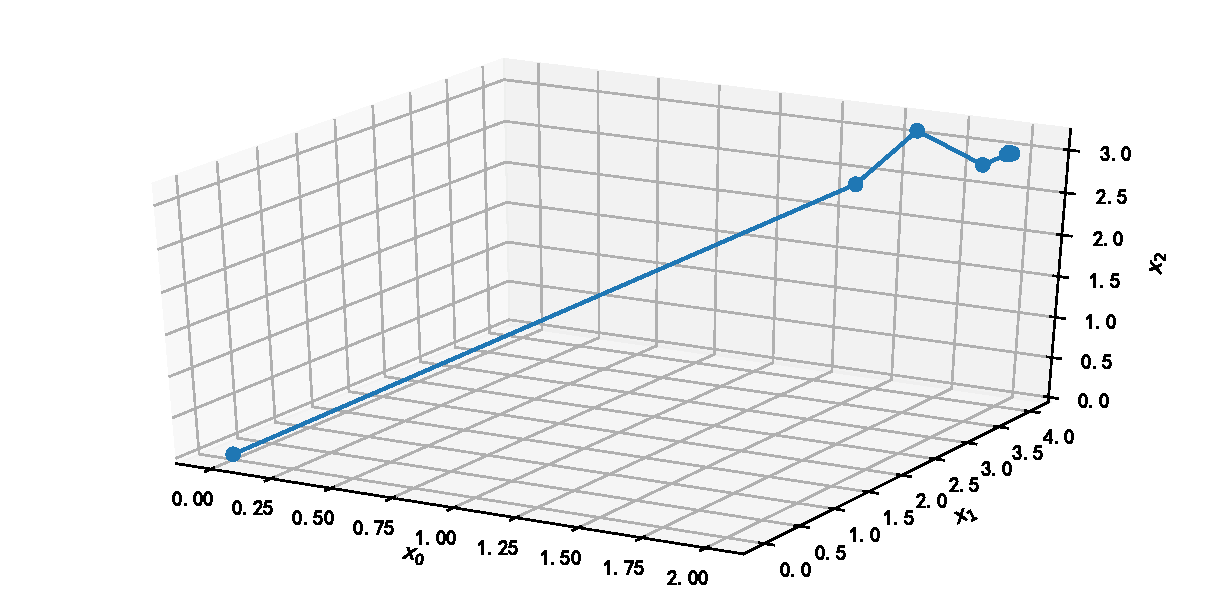
\includegraphics[width=\linewidth]{fig13.pdf}
\end{figure}

\begin{figure}[H]
	\centering
	\caption{Jacobi迭代的每个解随迭代次数的变化}
	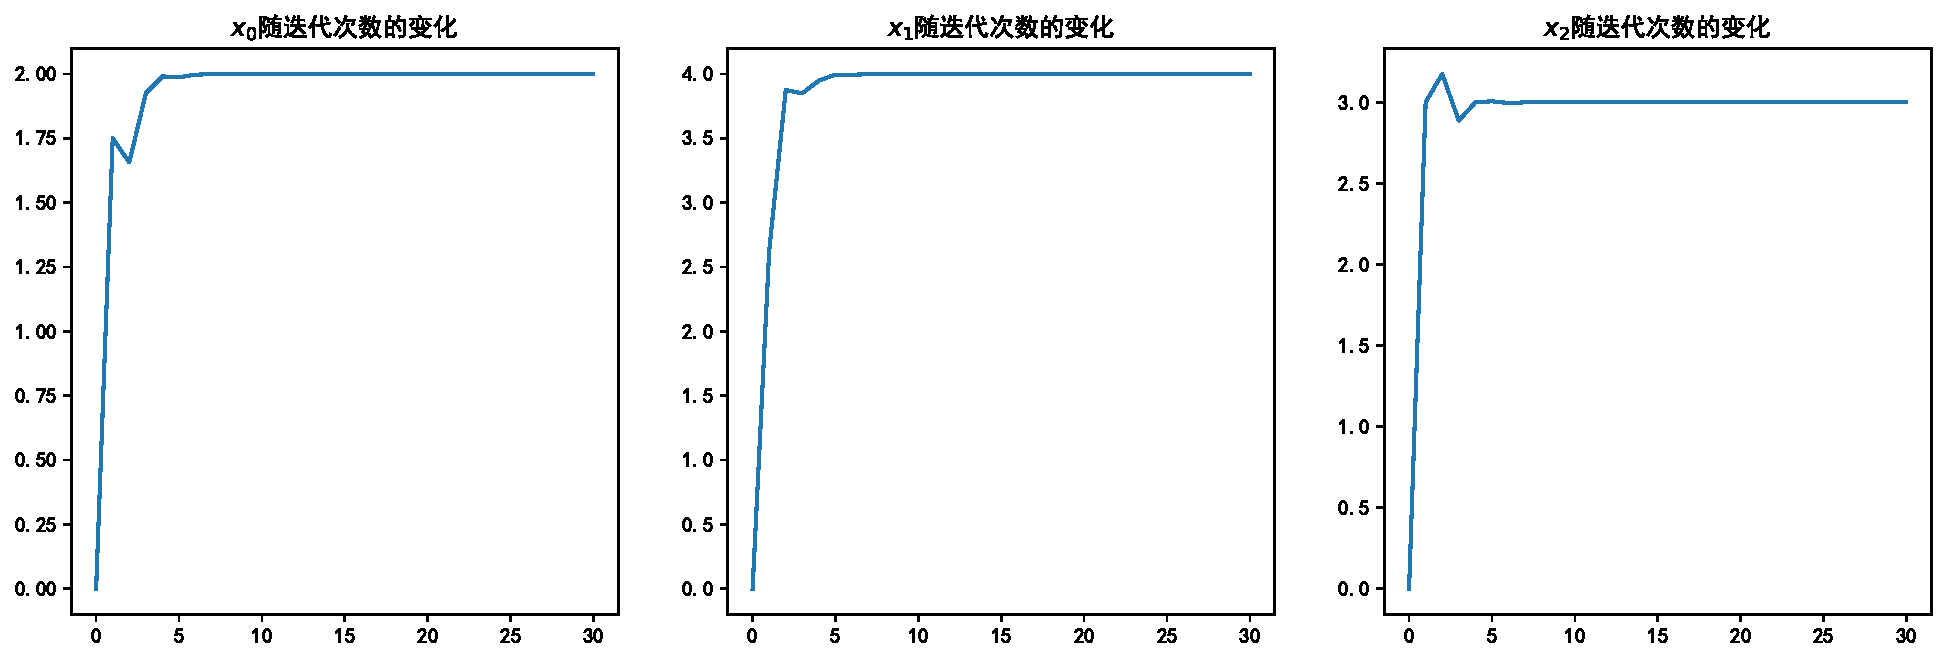
\includegraphics[width=\linewidth]{fig14.pdf}
\end{figure}


\paragraph{Jacobi迭代代码}
~\\
\begin{minted}[mathescape,
               linenos,
               numbersep=5pt,
               frame=lines,
               framesep=2mm]{python}
def jacobi(A, B, max_iter, x=None, ax=None):
    B = B.reshape(-1)
    if x is None:
        x = np.zeros_like(B)
    show = ax is not None and x.size == 3
    showx = [[] for _ in range(3)]
\end{minted}
\begin{minted}{python}
    D = np.diag(A)
    R = A - np.diagflat(D)
    if show:
        for i in range(len(showx)):
            showx[i].append(x[i])
    for _ in range(max_iter):
        x = (B - np.dot(R, x)) / D
        if show:
            for i in range(len(showx)):
                showx[i].append(x[i])
    if show:
        ax.plot(showx[0], showx[1], showx[2], marker='o')
        ax.set_xlabel('$x_0$')
        ax.set_ylabel('$x_1$')
        ax.set_zlabel('$x_2$')
        return x, np.array(showx)
    return x
\end{minted}

\paragraph{Gauss-Seidel方法}
~\\
如果把Jacobi迭代公式改成以下形式
$$\left\{
\begin{aligned}
x_1^{\left(k+1\right)} = \frac{1}{a_{11}}&\left(-a_{12}x_2^{\left(k\right)} -a_{13}x_3^{\left(k\right)} -\cdots - a_{1n}x_n^{\left(k\right)} +b_1\right) \\
x_2^{\left(k+1\right)} = \frac{1}{a_{22}}&\left(-a_{21}x_1^{\left(k+1\right)} -a_{23}x_3^{\left(k\right)} -\cdots - a_{2n}x_n^{\left(k\right)} +b_2\right) \\
&\vdots \\
x_n^{\left(k+1\right)} = \frac{1}{a_{nn}}&\left(-a_{n1}x_1^{\left(k+1\right)} -a_{n2}x_2^{\left(k+1\right)} -\cdots - a_{n,n-1}x_{n-1}^{\left(k+1\right)} +b_n\right) 
\end{aligned}
\right.$$
选取初始向量$\mathbf{x}^{\left(0\right)}$, 用迭代公式:
$$\left\{
\begin{aligned}
\mathbf{x}^{\left(0\right)} &= \left(x_1^{\left(0\right)},x_2^{\left(0\right),\cdots,x_n^{\left(0\right)}}\right)^T \\
x_i^{\left(k+1\right)} &= \frac{1}{a_{ii}}\left(b_i - \sum_{j=1}^{i-1}a_{ij}x_j^{\left(k+1\right)} - \sum_{j=i+1}^{n}a_{ij}x_j^{\left(k\right)} \right)
\end{aligned}
\right.$$
Gauss-Seidel迭代法也可以写为向量递推的形式:
$$\mathbf{x}^{\left(k\right)} = \mathbf{T}_g\mathbf{x}^{\left(k\right)} + \mathbf{c}_g$$
或
$$\left(\mathbf{D} - \mathbf{L}\right) \mathbf{x}^{\left(k\right)} = \mathbf{U} \mathbf{x}^{\left(k-1 \right)} + \mathbf{b}$$
即
$$ \mathbf{x}^{\left(k\right)} = \left(\mathbf{D} - \mathbf{L}\right)^{-1}\mathbf{U}\mathbf{x}^{k-1} + \left(\mathbf{D} - \mathbf{L}\right)^{-1}\mathbf{b}$$

由方程组可得:$x=\frac{7+y+z}{4}$,$y=\frac{21+4*x+z}{8}$,$z=\frac{15+2*x-y}{5}$
这样就提出了下列Gauss-Seidel迭代过程:

$$ \left\{
\begin{aligned}
x_{k+1}& =\frac{7+1*y_k+z_k}{4} \\
y_{k+1}& =\frac{21+4 * x_{k+1}+z_k}{8} \\
z_{k+1}& =\frac{15+2*x_{k+1}-y_{k+1}}{5}
\end{aligned}
\right.
$$

Jacobi方法没有利用刚计算出来的值,而Gauss-Seidel方法利用了刚计算出来的值,Gauss-Seildel方法对于相同的精度应该需要的迭代次数应该比Jacobi方法的要少,即收敛得更快。实际上因为有Stein-Rosenberg定理有:如果对每个$i≠j,a_{ij}≤0$,且对每个$i=1,2,…,n$ $ a_{ii}>0$,那么一下结论有且只有一个成立:

\begin{align*}
0 \leq p(T_g) < p(T_g) < 1\\
1 < p(T_j)<p(T_g)\\
p(T_j)=p(T_g)=0\\
p(T_j)=p(T_g)=1\\
\end{align*}

\paragraph{Gauss-Seidel方法的解随迭代次数的变化}

下面是Gauss-Seidel方法的解随迭代次数的变化表与变化图:

\begin{table}[H]
	\centering
	\caption{Gauss-Seidel方法的解随迭代次数的变化表}
	\begin{tabular}{llll}
		\hline
		迭代次数 & $x_0$          & $x_1$          & $x_2$          \\ \hline
0    & 0.000000000000 & 0.000000000000 & 0.000000000000 \\
1    & 1.750000000000 & 3.500000000000 & 3.000000000000 \\
2    & 1.875000000000 & 3.937500000000 & 2.962500000000 \\
3    & 1.993750000000 & 3.992187500000 & 2.999062500000 \\
4    & 1.998281250000 & 3.999023437500 & 2.999507812500 \\
5    & 1.999878906250 & 3.999877929688 & 2.999975976563 \\
6    & 1.999975488281 & 3.999984741211 & 2.999993247070 \\
7    & 1.999997873535 & 3.999998092651 & 2.999999530884 \\
$\cdots$ & $\cdots$  & $\cdots$  & $\cdots$ \\
24   & 2.000000000000 & 4.000000000000 & 3.000000000000 \\
25   & 2.000000000000 & 4.000000000000 & 3.000000000000 \\
26   & 2.000000000000 & 4.000000000000 & 3.000000000000 \\
27   & 2.000000000000 & 4.000000000000 & 3.000000000000 \\
28   & 2.000000000000 & 4.000000000000 & 3.000000000000 \\
29   & 2.000000000000 & 4.000000000000 & 3.000000000000 \\ \hline
	\end{tabular}
\end{table}

\begin{figure}[H]
	\centering
	\caption{Gauss-Seidel方法的解随迭代次数的变化}
	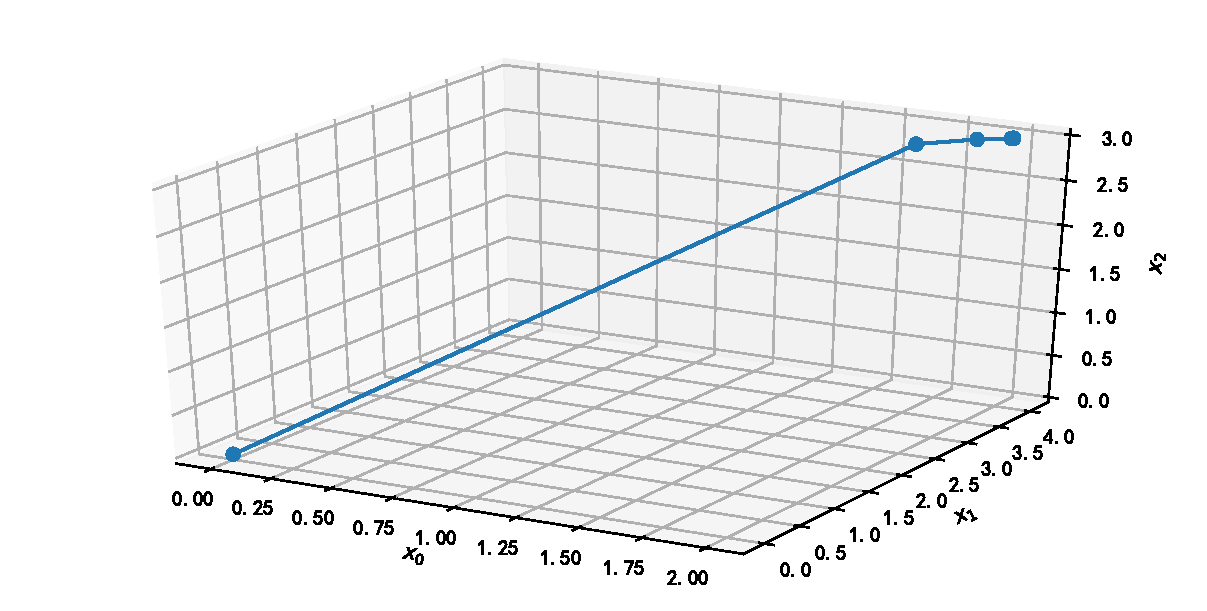
\includegraphics[width=\linewidth]{fig15.pdf}
\end{figure}

\begin{figure}[H]
	\centering
	\caption{Gauss-Seidel方法的每个解随迭代次数的变化}
	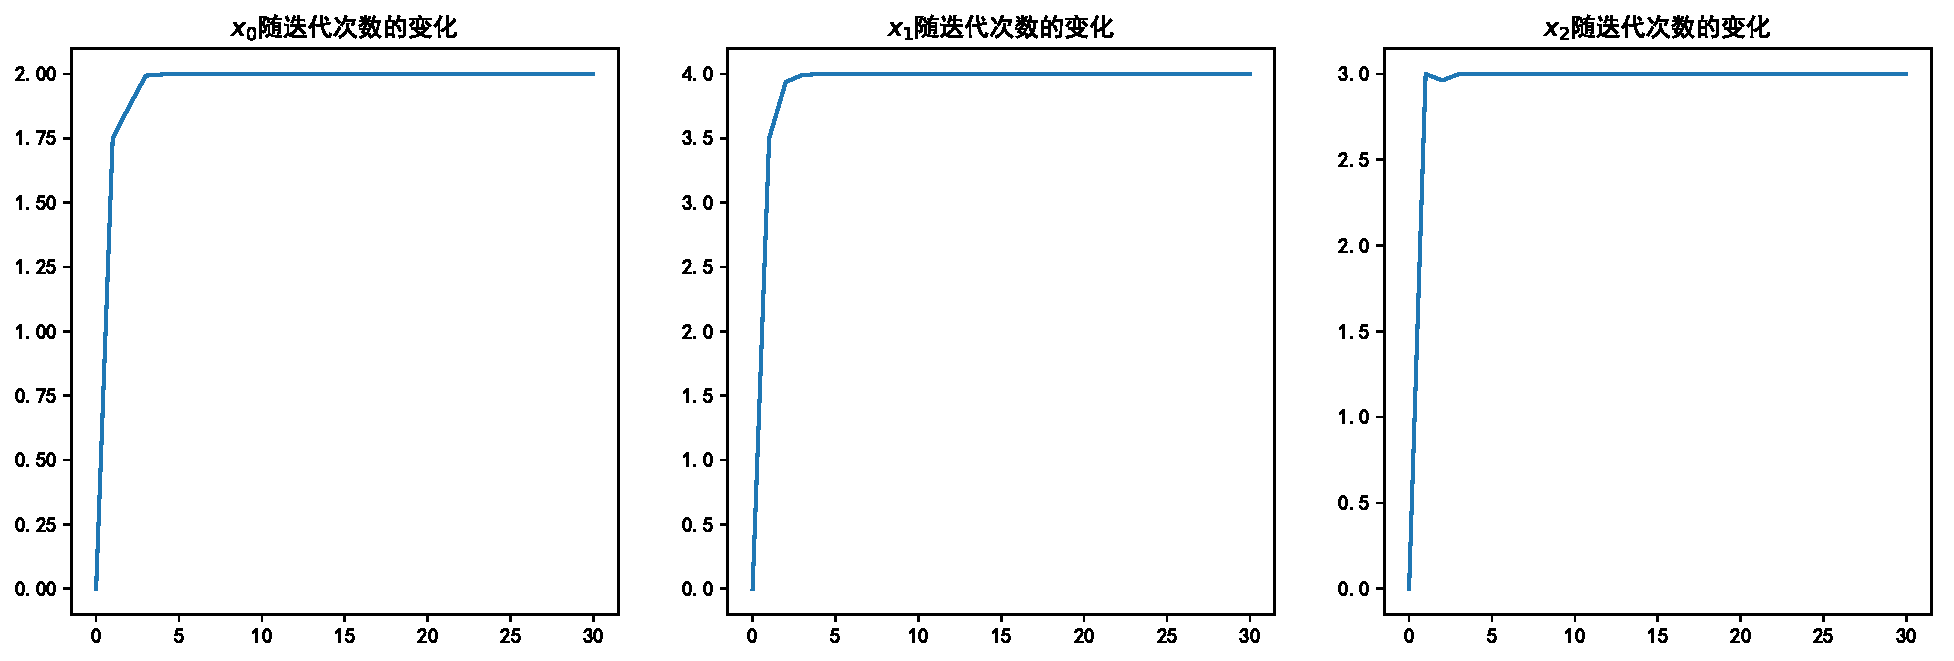
\includegraphics[width=\linewidth]{fig16.pdf}
\end{figure}

\paragraph{Gauss-Seidel方法代码}
~\\
\begin{minted}{python}
def gauss_seidel(A, B, max_iter, x=None, ax=None):
    B = B.reshape(-1)
    if x is None:
        x = np.zeros_like(B)
    show = ax is not None and x.size == 3
    showx = [[] for _ in range(3)]
\end{minted}
\begin{minted}{python}
    if show:
        for i in range(len(showx)):
            showx[i].append(x[i])
    for _ in range(max_iter):
        x_new = np.zeros_like(x)
        for i in range(A.shape[0]):
            s1 = np.dot(A[i, :i], x_new[:i])
            s2 = np.dot(A[i, i + 1:], x[i + 1:])
            x_new[i] = (B[i] - s1 - s2) / A[i, i]
        x = x_new
        if show:
            for i in range(len(showx)):
                showx[i].append(x[i])
    if show:
        ax.plot(showx[0], showx[1], showx[2], marker='o')
        ax.set_xlabel('$x_0$')
        ax.set_ylabel('$x_1$')
        ax.set_zlabel('$x_2$')
        return x, np.array(showx)
    return x
\end{minted}

\paragraph{Jacobi迭代与Gauss-Seidel方法对比}
~\\
下图是Jacobi迭代与Gauss-Seidel方法在每个解上的对比图:

\begin{figure}[H]
	\centering
	\caption{Jacobi迭代与Gauss-Seidel方法对比图}
	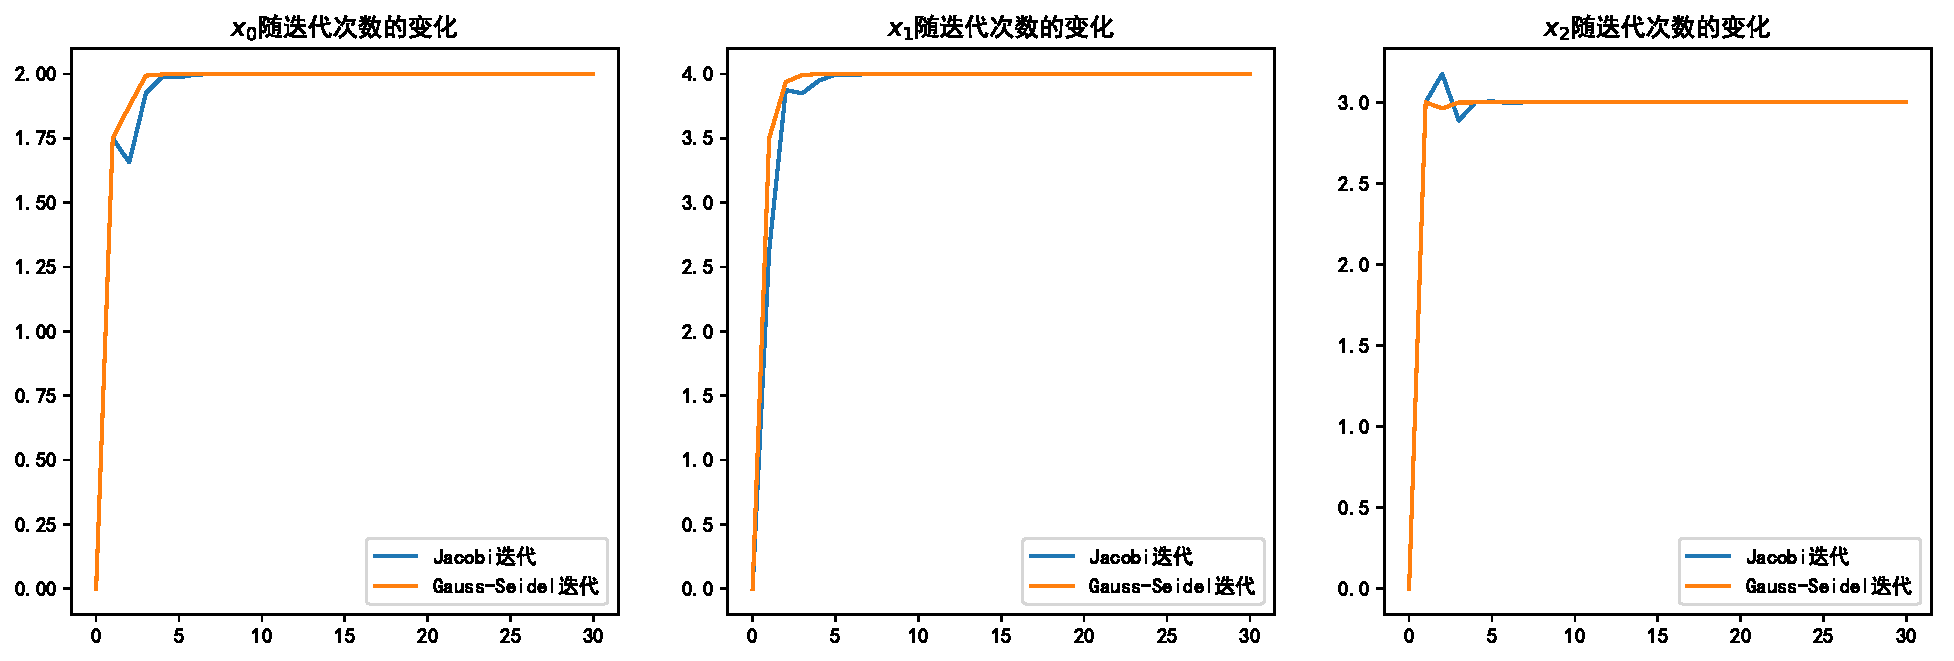
\includegraphics[width=.9\linewidth]{fig17.pdf}
\end{figure}

\subsection{题目2}

设有如下三角线性方程组,而且系数矩阵具有严格对角优势:

$$
\begin{matrix}
d_1x_1 &+&c_1x_2 &  & & & & &=&b_1\\
a_1x_1 &+& d_2x_2&+& c_2x_3 & & & &=&b_2\\
& & a_2x_2 &+& d_3x_3 &+& c_3x_4 & &=&b_3\\
& & . & & & &&&.\\
& &  &. & & &&&.\\
& & & &. & &&&.\\
& & & &  & a_{N-1}x_{N-1}&+&d_Nx_N&=&b_N\\
\end{matrix}
$$

设计一个算法来求解上述方程组. 算法必须有效地利用系数矩阵的稀疏性。

\paragraph{分析}
~\\
对第一行$d_xx_1 +c_1x_2 = b$,将其转变为$x_1 + \frac{c_1}{d_1}x_2 = \frac{b_1}{d_1}$

对将第一行乘$a_1$与第二行相减,把第二行转变为\[(d_2 - \frac{a_1c_1}{d_1})x_2 + c_2x_3 = \frac{c_2}{d_2} - \frac{a_2b_1}{d_1}\]

然后用第二行转化第三行,第三行转化第四行,以此类推。最终矩阵的形式为
\begin{align*}
\begin{pmatrix}
1 & r_1 & &  & \\ 
& 1 & \ddots & & \\ 
&  & 1 & \ddots & \\ 
&  &  & \ddots & r_1\\ 
&  &  &  & 1
\end{pmatrix}
\begin{pmatrix}
x_1\\ 
x_2\\ 
\vdots\\ 
x_{n-1}\\
x_n
\end{pmatrix}
=
\begin{pmatrix}
\rho_1\\ 
\rho_2\\ 
\vdots\\ 
\rho_{n-1}\\
\rho_n
\end{pmatrix}
\end{align*}

三对角矩阵是容易求解的。无论是多大的矩阵,利用托马斯算法我们可以仅仅使用两次迭代就求出了精确的解。如果使用迭代算法Guass-Seidel算法往往需要数十次的迭代。所以利用矩阵的稀疏性可以大大提高求解的效率。

\subsection{题目3}

利用Gauss-Seidel迭代法求解下列带状方程。

\[AX = B\]

其中,
\begin{align*}
A = \begin{bmatrix}
12. & -2. & 1. & ... & 0. & 0. & 0.\\
-2. & 12. & -2. & ... & 0. & 0. & 0.\\
1. & -2. & 12. & ... & 0. & 0. & 0.\\
...\\
0. & 0. & 0. & ... & 12. & -2. & 1.\\
0. & 0. & 0. & ... & -2. & 12. & -2.\\
0. & 0. & 0. & ... & 1. & -2. & 12.\\
\end{bmatrix}
B = \begin{bmatrix} 5.\\5.\\5.\\...\\5.\\5.\\5.\\ \end{bmatrix}
\end{align*}

使用Gauss-Seidel方法解得
\begin{align*}
X = \begin{bmatrix}
0.46379552 & 0.53728461 & 0.50902292 & 0.49822163 & 0.49894186 & 0.49998535\\
0.50008872 & 0.50001532 & 0.49999479 & 0.49999786 & 0.50000011 & 0.5000002\\
0.50000002 & 0.49999999 & 0.5 & 0.5 & 0.5 & 0.5\\
0.5 & 0.5 & 0.5 & 0.5 & 0.5 & 0.5\\
0.5 & 0.5 & 0.5 & 0.5 & 0.5 & 0.5\\
0.5 & 0.5 & 0.5 & 0.5 & 0.5 & 0.5\\
0.49999999 & 0.50000002 & 0.5000002 & 0.50000011 & 0.49999786 & 0.49999479\\
0.50001532 & 0.50008872 & 0.49998535 & 0.49894186 & 0.49822163 & 0.50902292\\
0.53728461 & 0.46379552\\
\end{bmatrix}
\end{align*}

\paragraph{Gauss-Seidel方法求解代码}
~\\
\begin{minted}{python}
A = 12 * np.identity(50)
for i in range(50):
    if i + 1 < 50: A[i][i + 1] = -2
    if i + 2 < 50: A[i][i + 2] = 1
    if i - 1 >= 0: A[i][i - 1] = -2
    if i - 2 >= 0: A[i][i - 2] = 1
B = 5 * np.ones(50).reshape(-1, 1)
x = gauss_seidel(A, B, 30)
\end{minted}

\section{第四章}



\subsection{题目1}

以$y=sin(x)$为例,在$[0,\pi]$区间内生成11个、21个数据点,设计算法或程序,用上述四个边界条件(自然边界、固定边界、周期边界、强制第一个子区间和第二个子区间样条多项式的三阶导数相等,倒数第二个子区间和最后一个子区间的三次样条函数的三阶导数相等),分别计算其样条插值,并作图比较,分析其差异性。

\paragraph{样条插值}

顾名思义,分段就是把区间$[a,b]$分成n个区间,共有n+1个点,其中两个端点$x_0=a,x_n=b$。三次样条就是说每个小区间的曲线是一个三次方程,三次样条方程满足以下条件:

1,在每个分段小区间$[x_i,x_{i+1}]$上, $S(x)=S_i(x)$都是一个三次方程

2,满足插值条件,即$S(x_i)=y_i \quad (i=0,1,\cdots ,n)$

3, 曲线光滑,即 $S(x),S'(x),S''(x)$ 连续

则这个三次方程可以构造成如下形式:

$y=a_i+b_i x+c_i x^2+d_i x^3$ 这种形式,我们称这个方程为三次样条函数 $S_i(x)$ 。

从 $S_i(x)$ 可以看出每个小区间有四个未知数 $(a_i,b_i,c_i,d_i)$ ,有n个小区间,则有4n个未知数,要解出这些未知数,则我们需要4n个方程来求解。

\paragraph{自然边界(Natural Spline)}

指定端点二阶导数为0,$S''(x_0)=0=S''(x_n)$


\paragraph{固定边界(Clamped Spline)}

指定端点一阶导数,这里分别为A和B,即$S'_0=A, S'_{n-1}(x_n)=B$

\paragraph{非扭结边界(Not-A-Knot Spline)}

强制第一个插值点的三阶导数值等于第二个点的三阶导数值,最后第一个点的三阶导数值等于倒数第二个点的三阶导数值. 即$S'''_0(x_0)=S'''_1(x_1) \quad and \quad S'''_{n-2}(x_{n-1})=S'''_{n-1}(x_n)$

\paragraph{周期边界(Periodic Spline)}

要求样条S(x)及其导函数是以区间长度$x_n-x_0$为周期的函数,即$S(x_0)=S(x_n),S'(x_0)=S'(x_n),S''(x_0)=S''(x_n)$

\paragraph{绘图}

分别将$[0,\pi]$等分成11段与21段,带入写好的样条插值函数中,计算对应的样条插值。然后,在$[0,\pi]$区间内,均匀的去50个点并将其映射到坐标轴上,得到如下两图:


\begin{figure}[H]
\centering
\begin{minipage}[t]{0.48\textwidth}
\centering
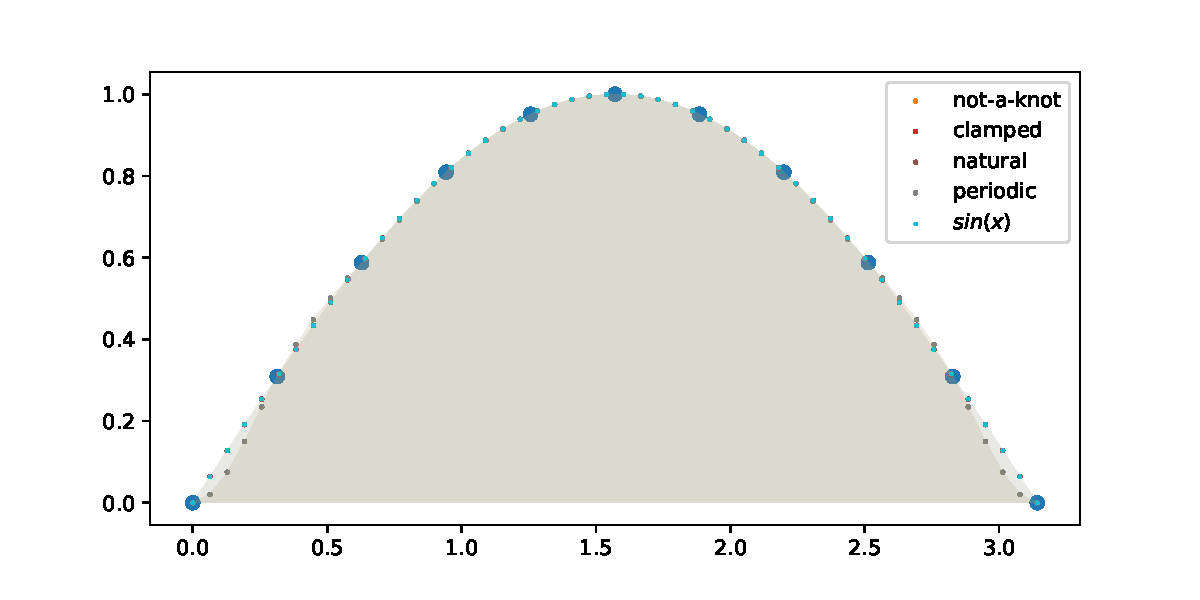
\includegraphics[width=6cm]{4-1.pdf}
\caption{$[0,\pi]$等分11段插值结果}
\end{minipage}
\begin{minipage}[t]{0.48\textwidth}
\centering
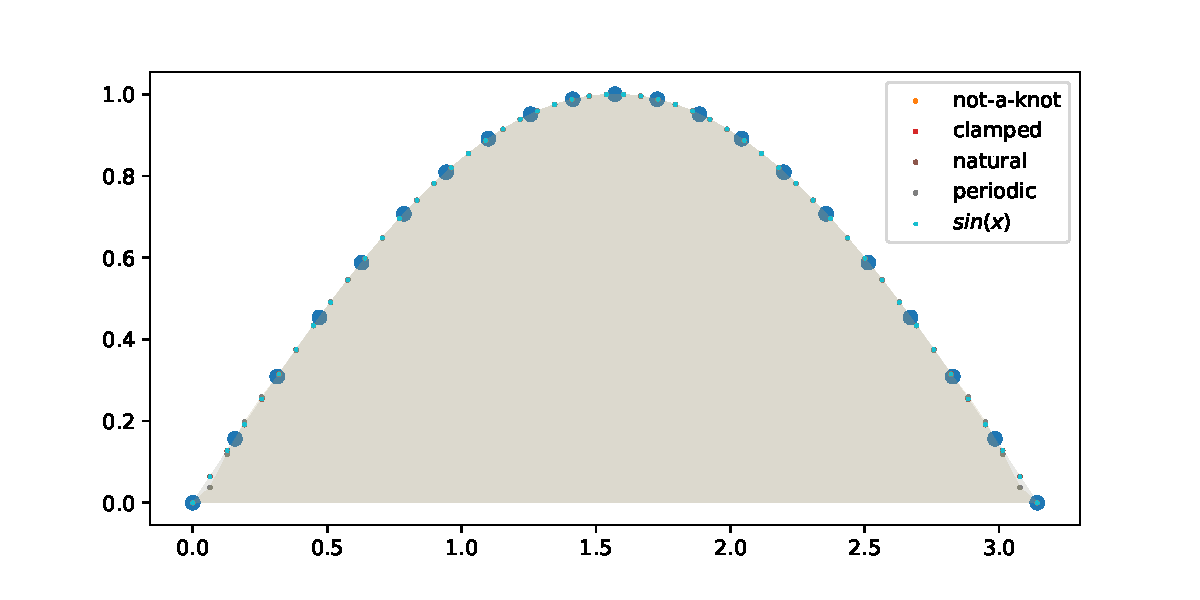
\includegraphics[width=6cm]{4-3.pdf}
\caption{$[0,\pi]$等分21段插值结果}
\end{minipage}
\end{figure}

可以观察到,由于三次拟合的情况较为良好,很难观察出不同节点之间的拟合情况,于是通过选择不同的映射点的个数,绘制下图

\begin{figure}[H]
	\centering
	\caption{不同边界条件插值绘制结果}
	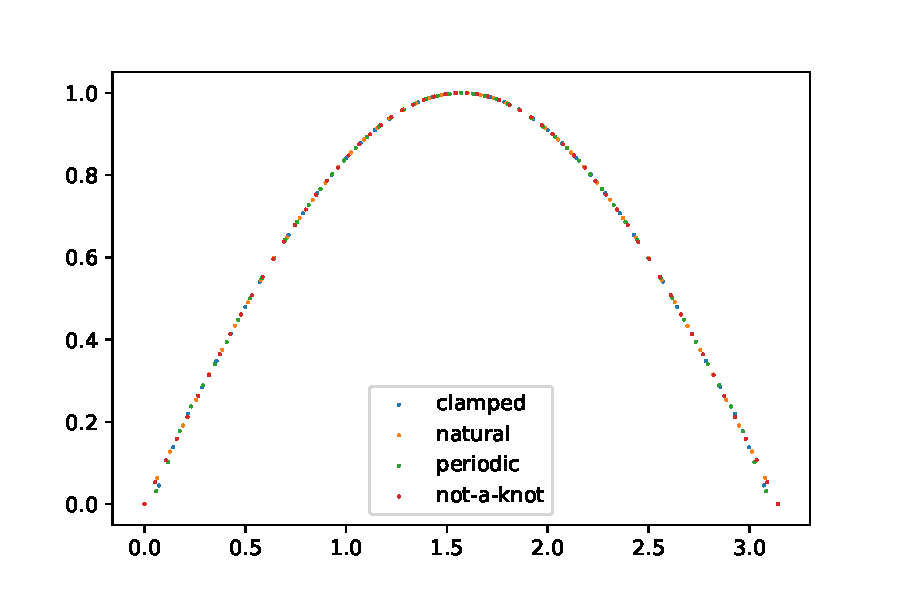
\includegraphics[width=.9\linewidth]{4-4.pdf}
\end{figure}

\paragraph{计算结果展示}


为了更好地展示所计算样条插值的结果,我们选取了插值计算后的前十个点,进行展示。下图是$[0,\pi]$区间内,选取50个点,前十个点经过sin(x)函数和不同边界条件的样条插值函数的计算结果


\begin{table}[H]
	\centering
	\caption{不同边界条件的样条插值函数的计算结果}
	\begin{tabular}{lllll}
		\hline
		sin         & clamped     & natural     & periodic    & not-a-knot  \\ \hline
		0           & 0           & 0           & 0           & 0           \\
		0.058144829 & 0.017166528 & 0.058141909 & 0.017166528 & 0.058212405 \\
		0.116092914 & 0.062694079 & 0.116088532 & 0.062694079 & 0.116180395 \\
		0.173648178 & 0.1276246   & 0.173644584 & 0.1276246   & 0.17372376  \\
		0.230615871 & 0.203000041 & 0.230614781 & 0.203000041 & 0.230662291 \\
		0.286803233 & 0.279862351 & 0.286803836 & 0.279862351 & 0.286815778 \\
		0.342020143 & 0.34965416  & 0.342017152 & 0.34965416  & 0.342004013 \\
		0.396079766 & 0.409813501 & 0.39607043  & 0.409813501 & 0.396046786 \\
		0.44879918  & 0.462393675 & 0.448787296 & 0.462393675 & 0.448763886 \\
		0.5         & 0.509566705 & 0.49999158  & 0.509566705 & 0.499975106 \\ \hline

	\end{tabular}
\end{table}



\paragraph{三次样条插值代码}


\begin{minted}{python}
def calculateEquationParameters(x):
    # parameter为二维数组,用来存放参数,sizeOfInterval是用来存放区间的个数
    parameter = []
    sizeOfInterval = len(x)-1
    i = 1
    # 首先输入方程两边相邻节点处函数值相等的方程为2n-2个方程
    while i < len(x)-1:
        data = init(sizeOfInterval*4)
        data[(i-1)*4] = x[i]*x[i]*x[i]
        data[(i-1)*4+1] = x[i]*x[i]
        data[(i-1)*4+2] = x[i]
        data[(i-1)*4+3] = 1
        data1 = init(sizeOfInterval*4)
        data1[i*4] = x[i]*x[i]*x[i]
        data1[i*4+1] = x[i]*x[i]
        data1[i*4+2] = x[i]
        data1[i*4+3] = 1
        temp = data[2:]
        parameter.append(temp)
        temp = data1[2:]
        parameter.append(temp)
        i += 1
   # 输入端点处的函数值。为两个方程, 加上前面的2n - 2个方程,一共2n个方程
    data = init(sizeOfInterval * 4 - 2)
    data[0] = x[0]
    data[1] = 1
    parameter.append(data)
    data = init(sizeOfInterval * 4)
    data[(sizeOfInterval - 1) * 4] = x[-1] * x[-1] * x[-1]
    data[(sizeOfInterval - 1) * 4 + 1] = x[-1] * x[-1]
    data[(sizeOfInterval - 1) * 4 + 2] = x[-1]
    data[(sizeOfInterval - 1) * 4 + 3] = 1
    temp = data[2:]
    parameter.append(temp)
    # 端点函数一阶导数值相等为n-1个方程。加上前面的方程为3n-1个方程。
    i = 1
    while i < sizeOfInterval:
        data = init(sizeOfInterval * 4)
        data[(i - 1) * 4] = 3 * x[i] * x[i]
        data[(i - 1) * 4 + 1] = 2 * x[i]
        data[(i - 1) * 4 + 2] = 1
        data[i * 4] = -3 * x[i] * x[i]
        data[i * 4 + 1] = -2 * x[i]
        data[i * 4 + 2] = -1
        temp = data[2:]
        parameter.append(temp)
        i += 1
    # 端点函数二阶导数值相等为n-1个方程。加上前面的方程为4n-2个方程。
    且端点处的函数值的二阶导数为零,为两个方程。总共为4n个方程。
    i = 1
    while i < len(x) - 1:
        data = init(sizeOfInterval * 4)
        data[(i - 1) * 4] = 6 * x[i]
        data[(i - 1) * 4 + 1] = 2
        data[i * 4] = -6 * x[i]
        data[i * 4 + 1] = -2
        temp = data[2:]
        parameter.append(temp)
        i += 1
    return parameter


"""
对一个size大小的元组初始化为0
"""


def init(size):
    j = 0
    data = []
    while j < size:
        data.append(0)
        j += 1
    return data


"""
功能:计算样条函数的系数。
参数:parametes为方程的系数,y为要插值函数的因变量。
返回值:三次插值函数的系数。
"""


def solutionOfEquation(parametes, y):
    sizeOfInterval = len(x) - 1
    result = init(sizeOfInterval*4-2)
    i = 1
    while i < sizeOfInterval:
        result[(i-1)*2] = y[i]
        result[(i-1)*2+1] = y[i]
        i += 1
    result[(sizeOfInterval-1)*2] = y[0]
    result[(sizeOfInterval-1)*2+1] = y[-1]
    a = np.array(calculateEquationParameters(x))
    b = np.array(result)
    for data_x in b:
        print(data_x)
    return np.linalg.solve(a, b)


"""
功能:根据所给参数,计算三次函数的函数值:
参数:parameters为二次函数的系数,x为自变量
返回值:为函数的因变量
"""


def calculate(paremeters, x):
    result = []
    for data_x in x:
        result.append(paremeters[0]*data_x*data_x*data_x+paremeters[1]
                      * data_x*data_x+paremeters[2]*data_x+paremeters[3])
    return result


"""
功能:将函数绘制成图像
参数:data_x,data_y为离散的点.new_data_x,
new_data_y为由拉格朗日插值函数计算的值。x为函数的预测值。
返回值:空
"""


def Draw(data_x, data_y, new_data_x, new_data_y):
    plt.plot(new_data_x, new_data_y, label="拟合曲线", color="black")
    plt.scatter(data_x, data_y, label="离散数据", color="red")
    mpl.rcParams['font.sans-serif'] = ['SimHei']
    mpl.rcParams['axes.unicode_minus'] = False
    plt.title("三次样条函数")
    plt.legend(loc="upper left")
    plt.show()
\end{minted}









\pagebreak
\section{第五章}



\subsection{题目1}

自行编写复合梯形公式、Simpson公式的计算程序 \footnote{注:本题为验证公式的正确性,选用《数值方法》课本例题作为验证,验证程序的正确性。该题目的要求为,$y=2+sin(2\sqrt{x})$,设立10个区间(即11个点),计算从1到6的积分值。}


\paragraph{组合梯形公式}

设函数划分宽度为$h$,一共有$M+1$个点,即$M$个区间。考虑到计算的简便性,采用以下公式计算函数的积分值
$$T(f,h)=\frac{h}{2}(f(a)+f(b))+h\sum_{k=1}^{M-1} f(x_k)$$

经过计算,对$y=2+sin(2\sqrt{x})$的积分值为:8.193854565172531

\paragraph{Simpson公式}

设一共有2M个区间,每个区间等距,距离为$h$,选用组合辛普森公式公式一进行计算,即
$$S(f,h)=\frac{h}{3}\sum_{k=1}^{M}(f(x_{2k-2})+4f(x_{2k-1})+f(x_{2k}))$$

经过计算,对$y=2+sin(2\sqrt{x})$的积分值为:8.183472811131802

\paragraph{代码}
\begin{minted}{python}
def trapezoid(f, a, b, M):
    sum = 0
    h = (b-a)/M
    # print(h)
    for i in range(1, M):
        sum += f(i*h+a)
        # print(f(i*h+a))

    return (h/2)*(f(a)+f(b))+sum*h
    
    
def simpson(f, a, b, M):
    h = (b - a) / (2 * M)
    s = 0
    for k in range(1, M + 1):
        s += f(a + (2 * k - 2) * h) + 4 * f(a + (2 * k - 1) * h) + f(a + 2 * k * h)
    s *= h / 3
    return s


\end{minted}

\subsection{题目2}

取$h=0.01$,分别利用复合梯形公式和辛普森公式,计算定积分
$$I(x)=\frac{1}{\sqrt{2 \pi}} \int_{0}^{1} \exp ^{-\frac{x^{2}}{2}} \mathrm{d} x$$
试与精确解比较,说明两种格式的优劣。

\paragraph{解答}
通过对\textit{题目一}函数的调用,分别求得利用复合梯形公式和辛普森公式的积分解为:
\[
0.34134272963911727\]
\[
0.34134474607022336
\]

查表得,原函数的积分值为$\phi(1)-\phi(2)$,计算得
原函数积分的值为:
\[
	0.3413447460685431
\]
可知,辛普森公式的计算精度更高


\paragraph{代码}


\begin{minted}{python}


def trapezoid(f, a, b, M):
    sum = 0
    h = (b-a)/M
    # print(h)
    for i in range(1, M):
        sum += f(i*h+a)
        # print(f(i*h+a))

    return (h/2)*(f(a)+f(b))+sum*h

def simpson(f, a, b, M):
    h = (b - a) / (2 * M)
    s = 0
    for k in range(1, M + 1):
        s += f(a + (2 * k - 2) * h) + 4 * f(a + (2 * k - 1) * h) + f(a + 2 * k * h)
    s *= h / 3
    return s


def I_simpson(h):
    M=int(2/h)
    c=1/(math.sqrt(2*math.pi))
    print(c*simpson(g,0,1,M))
    
def I_trapezoid(h):
    M=int(1/h)
    c=1/(math.sqrt(2*math.pi))
    print(c*simpson(g,0,1,M))
    
I_simpson(0.01)
I_trapezoid(0.01)
\end{minted}






\subsection{题目3}
若取计算精度为$10^{-4}$,则h=?,n=?

\subsubsection{Simpson公式求解}
取h=0.5,n=2(原公式为M=1)时,求得的积分解为0.3415290519962957
取h=0.25,n=4(原公式为M=2)时,求得的积分为0.34135548785664915,误差$e=1.074178810606119e-05$小于$10^{-4}$。故精度为$10^{-4}$时,h=0.25,n=4;



\subsubsection{复合梯形公式求解}
取$h_0=0.01$,并依次增加,不断求出复合梯形公式的计算结果与精确解之间的误差,前10次迭代结果为:

$$h_{0}=0.01,I(x)=-0.000002016$$
$$h_{1}=0.02,I(x)=-0.000008066$$
$$h_{2}=0.03,I(x)=-0.000018517$$
$$h_{3}=0.04,I(x)=-0.000032265$$
$$h_{4}=0.05,I(x)=-0.000050415$$
$$h_{5}=0.06,I(x)=-0.000078777$$
$$h_{6}=0.07,I(x)=-0.000102896$$
$$h_{7}=0.08,I(x)=-0.000140062$$
$$h_{8}=0.09,I(x)=-0.000166692$$
$$h_{9}=0.10,I(x)=-0.000201710$$
$$h_{10}=0.11,I(x)=-0.000249044$$


即,当精度为$10^-4$时,h最大为0.06,但由于n不是整数,故h应取0.05,n应取20;











\section{第六章}

\subsection{题目1}

求$y'=1+y^2,y(0)=0$的数值解(分别用欧拉显格式、梯形预估修正格式、4阶龙格库塔格式,并与解析解比较这三种格式的收敛性)

\paragraph{欧拉显式格式}:
\subparagraph{公式推导}
根据泰勒展开, 有

$$y\left(t_{j+1}\right) + hf\left(t_j,y\left(t_j\right)\right) + \frac{h^2}{2}y^{''}\left(\xi_j\right)$$

忽略余项, 可以得到欧拉显式格式:

$$\left\{
\begin{aligned}
w_0 &= \alpha \\
w_{j+1} &= w_j + hf\left(t_j,w_j\right)
\end{aligned}
\right.$$

\subparagraph{误差分析}

假设 $f$在$D = \left\{\left(t,y\right) \big{|} a \leq t \leq b,-\infty < y < \infty \right\}$连续,满足Lipschitz条件(Lipschitz常数为$L$),且满足$\left|y^{''}\left(t\right) \right| \leq M,\forall t\in \left[a,b\right]$. 则$\left|y\left(t_j\right) - w_j \right| \leq \frac{hM}{2L}\left[ e^{L\left(t_j-a\right)}-1\right]$.在某些情况下, $M,L$较难确定. 但可以发现, 随着向后递推, 欧拉显式格式的误差逐渐增大。

\subparagraph{欧拉法误差分析}

对于$$\left|y\left(x_j\right) - w_j \right| \leq \frac{hM}{2L}\left[ e^{L\left(x_j-a\right)}-1\right]$$, 需要确定$M,L$的值.

由于$$M = \max \left|y^{''}\left(x\right) \right|,x\in \left[a,b\right]$$,

而$$y\left(x\right) = \sqrt{2x+1}$$,$$y^{''}\left(x\right) = \frac{-1}{\left(2x+1\right)^{3/2}}$$

有$$M = \max \left|y^{''}\left(x\right) \right| = \left|f^{''}\left(-1\right)\right| = 1$$

$$ \frac{\partial f}{\partial y} = 1+\frac{2x}{y^2} = 1+\frac{2x}{1+2x}$$, $$L = \max \left|\frac{\partial f}{\partial y} \right| = \left|\frac{\partial f}{\partial y} \big{|}_{x=1} \right| \approx 1.6667$$.

因此$$\left|y\left(1\right) - w_{n} \right| \leq \frac{hM}{2L}\left[ e^{L}-1\right] $$。

\paragraph{梯形预估修正格式}

利用数值积分方法将微分方程离散化时,若用梯形公式计算右端积分,即
$$\int_{x_{n}}^{x_{m 1}} f(x, y(x)) d x \approx \frac{h}{2}\left[f\left(x_{n}, y\left(x_{n}\right)\right)+f\left(x_{n+1}, y\left(x_{n+1}\right)\right)\right]$$
并用$y_n,y_{n+1}$代替$y(x_n),y(x_{n+1})$,则得计算公式
$$y_{n+1}=y_{n}+\frac{h}{2}\left[f\left(x_{n}, y_{n}\right)+f\left(x_{n+1}, y_{n+1}\right)\right]$$
这就是梯形预估修正格式。由于梯形公式仍是隐式格式,一般需用迭代法求解,迭代公式为

$$\left \{ \begin{array}{l}{y_{n+1}^{(0)}=y_{n}+h f\left(x_{n}, y_{n}\right)} \\ {y_{n+1}^{(k+1)}=y_{n}+\frac{h}{2}\left[f\left(x_{n}, y_{n}\right)+f\left(x_{n+1}, y_{n+1}^{(k)}\right)\right]} \\ {(k=0,1,2, \cdots)}\end{array}\right.$$

\paragraph{4阶龙格库塔格式}

对于方程$y'=f(x)$,存在a,其中$x_n<a<x_{n+1}$,有$\frac{y(x_{n+1})-y(x_n)}{h}=y'=f(x)$,为了提高y的精度,我们令
$$K_1=f(x_n,y_n)$$$$K_2=f(x_{n+\frac{1}{2}},y_n+\frac{h}{2}K_1)$$$$K_3=f(x_{n+\frac{1}{2}},y_n+\frac{h}{2}K_1)$$$$K_4=f(x_{n+1},y_n+hK_3)$$$$y_{n+1}=y_n+\frac{h}{6}(K_1+2K_2+2K_3+K_4)$$


\paragraph{解答}


使用欧拉显格式对于$y'=1+y^2,y(0)=0$求数值解得下拟合图:

\begin{figure}[H]
	\centering
	\caption{欧拉显格式}
	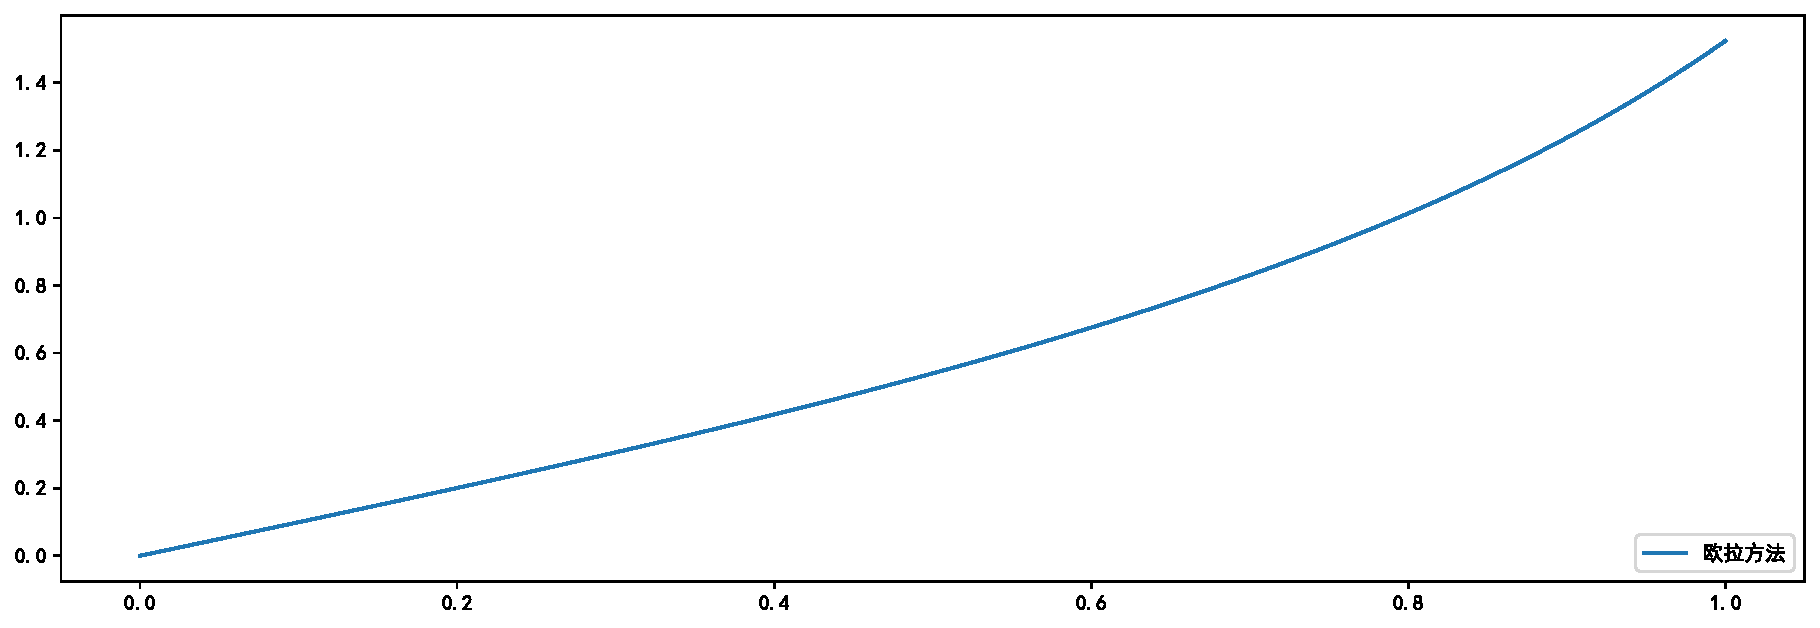
\includegraphics[width=\linewidth]{6-1.pdf}
\end{figure}

使用4阶龙格库塔格式对于$y'=1+y^2,y(0)=0$求数值解得下拟合图:

\begin{figure}[H]
	\centering
	\caption{4阶龙格库塔格式}
	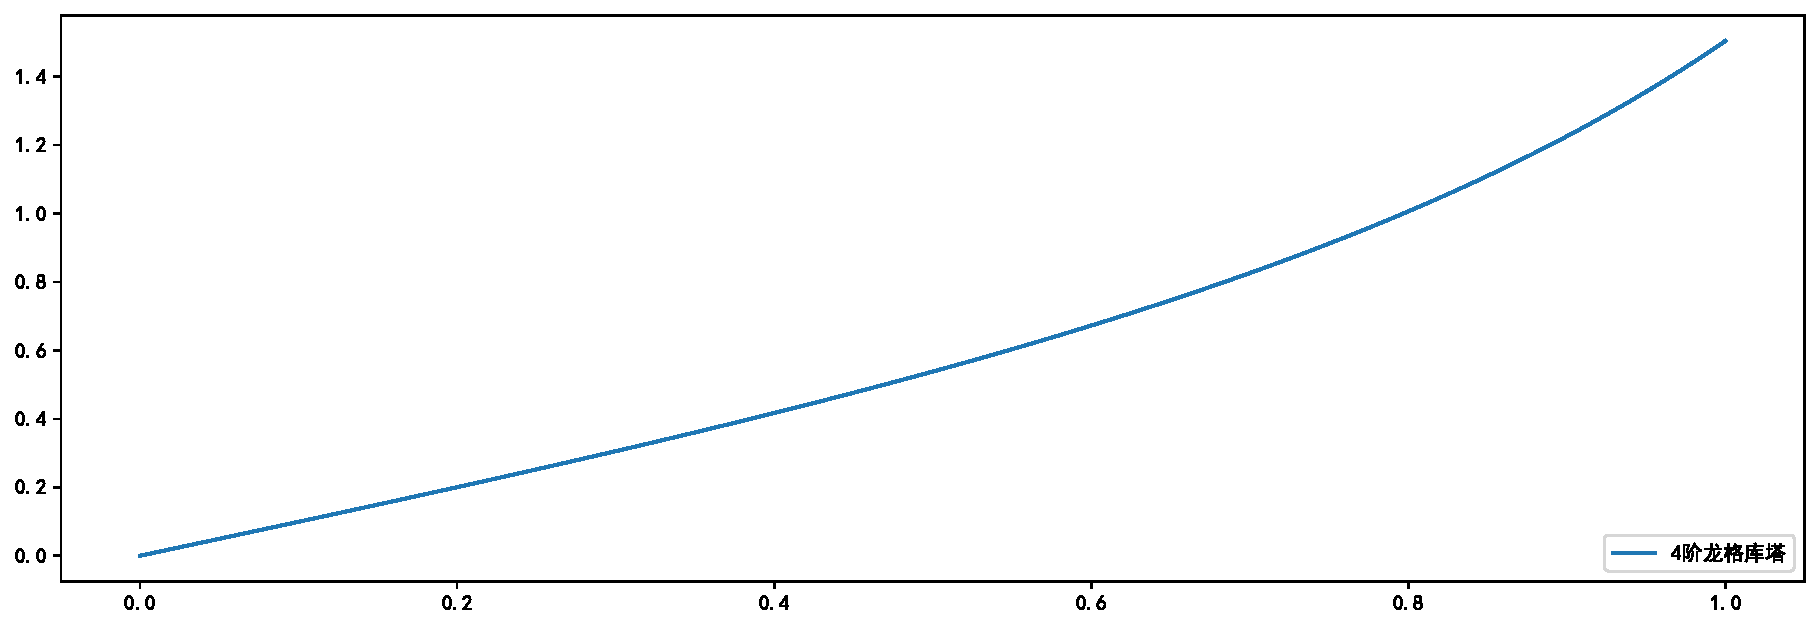
\includegraphics[width=\linewidth]{6-2.pdf}
\end{figure}

使用梯形预估修正格式对于$y'=1+y^2,y(0)=0$求数值解得下拟合图:

\begin{figure}[H]
	\centering
	\caption{梯形预估修正格式}
	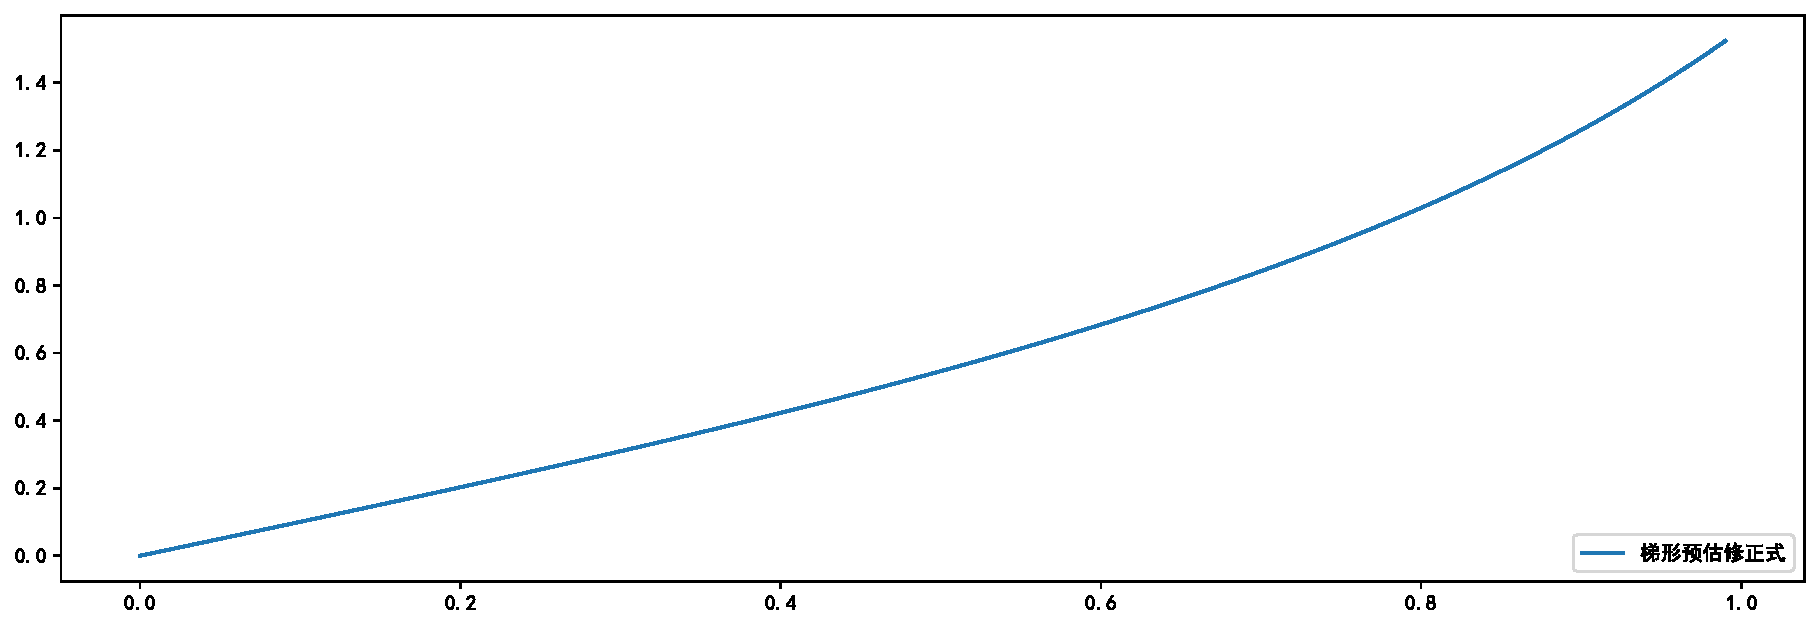
\includegraphics[width=\linewidth]{6-3.pdf}
\end{figure}






对方程求解得,y=tan(x).取h=0.01,分别利用欧拉显格式、梯形预估修正格式和4阶龙格库塔格式计算对应的解,绘制下图:


\begin{figure}[H]
	\centering
	\caption{3种方法与原函数的图像}
	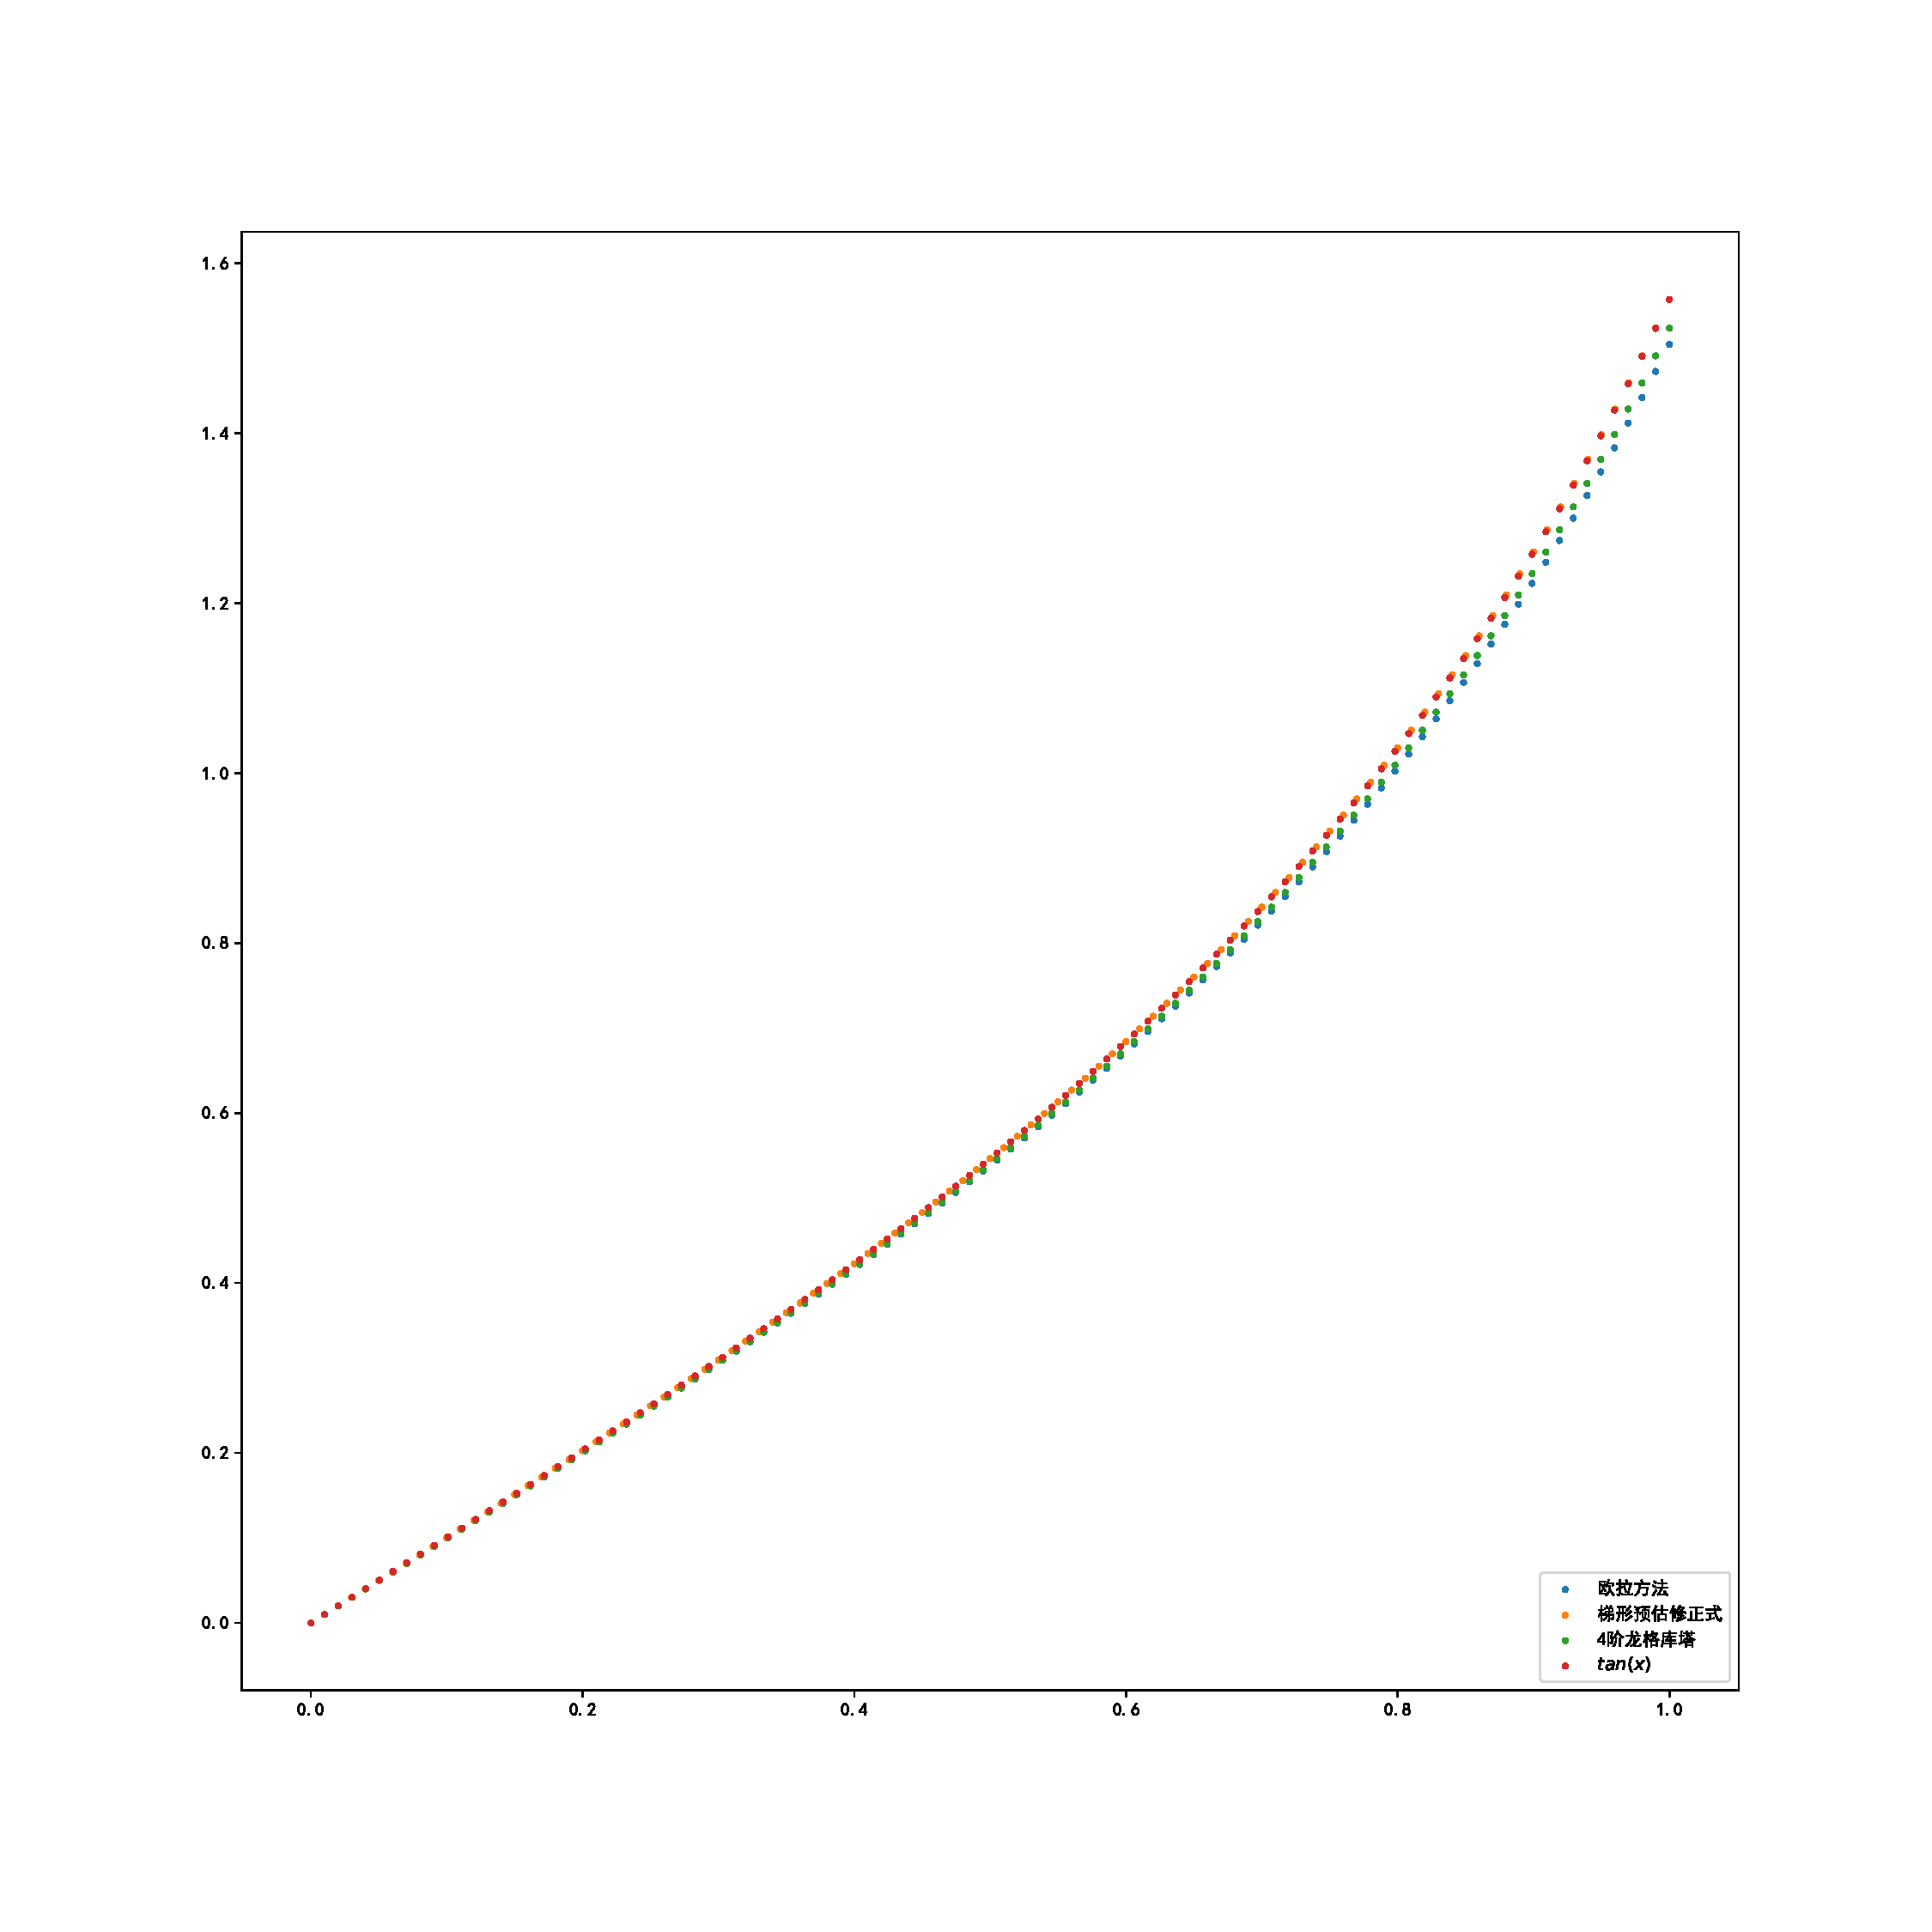
\includegraphics[width=\linewidth]{6-4.pdf}
\end{figure}


\paragraph{代码}

\begin{minted}{python}

def f(y):
    return 1+y**2


def euler(t, y0, a, b):
    t = np.linspace(a, b, M)
    y = np.zeros(M)
    y[0] = y0
    for k in range(M - 1):
        y[k + 1] = y[k] + h * f(y[k])
        
def rk4(f, a, b, ya, M):
    h = (b - a) / M
    T = np.linspace(a, b, M)
    Y = np.zeros(M)
    Y[0] = ya
    for j in range(M - 1):
        k1 = h * f(T[j], Y[j])
        k2 = h * f(T[j] + h / 2, Y[j] + k1 / 2)
        k3 = h * f(T[j] + h / 2, Y[j] + k2 / 2)
        k4 = h * f(T[j] + h, Y[j] + k3)
        Y[j + 1] = Y[j] + (k1 + 2 * k2 + 2 * k3 + k4) / 6
    return T, Y

def improved_euler(f,a=0,b=1,ya=1,h=0.1,verbose=True):
    res = []
    xi = a 
    yi = ya
    
    
    while xi <= b: # 在求解区间范围
        yp = yi + h*f(xi, yi)
        y = yi + h/2 * (f(xi, yi) + f(xi, yp))
        if verbose:
            xxx.append(xi)
            yyy.append(yi)
            #print('xi:{:.4f}, yi:{:.6f}'.format(xi,yi))
        res.append(y)
        xi, yi = xi+h, y
    
    return res
    
plt.figure(figsize=(15, 15))
#plt.subplot(1, 2, 1)
#T, Y = rk4(f, 0, 1.0, 0, 1000)
x=np.linspace(0,1,100)
plt.scatter(t, y, label='欧拉方法',s=6)
plt.scatter(xxx, yyy, label='梯形预估修正式',s=6)
plt.scatter(T, Y, label='4阶龙格库塔',s=6)
plt.scatter(x, np.tan(x), label='$tan(x)$',s=6)
plt.legend(loc='lower right')
plt.savefig('6-4.pdf')

\end{minted}

\subsection{题目2}
用龙格库塔4阶方法求解描述振荡器的经典van der Pol微分方程
$$\left\{
\begin{aligned}
\frac{d^2y}{dt^2}-\mu(1-y^2)\frac{dy}{dt}+y=0,\\
y(0)=1,y'(0)=0
\end{aligned}
\right.$$
分别取$\mu=0.01,0.1,1$作图比较计算结果

\paragraph{解答}
通过python实现四阶龙格库塔方法并作图得:

\begin{figure}[H]
	\centering
	\caption{四阶龙格库塔方法}
	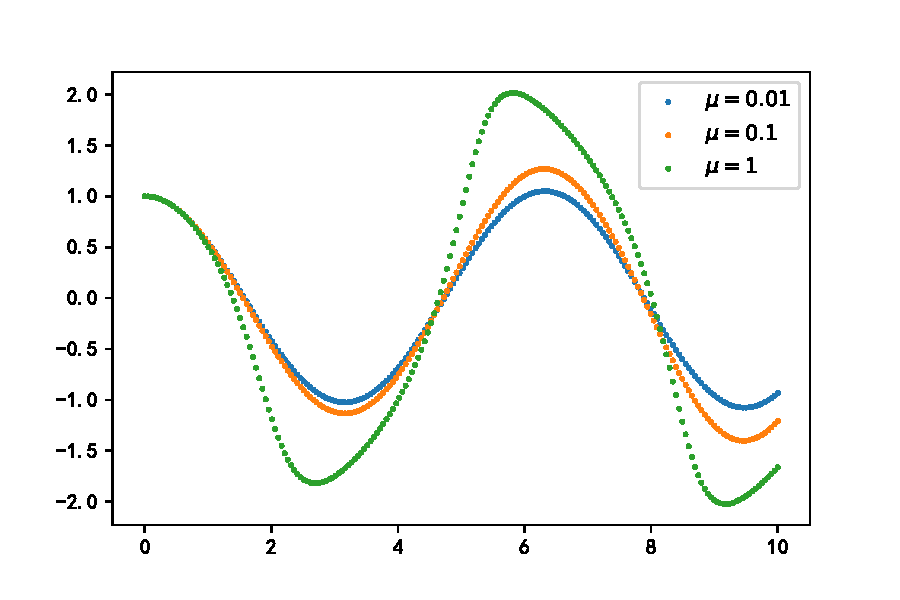
\includegraphics[width=\linewidth]{6-5.pdf}
\end{figure}

\paragraph{代码}


\begin{minted}{python}
def ff1(w1, w2):
    return 0.01*(1-w1*w1)*w2-w1

def ff2(w1, w2):
    return 0.1*(1-w1*w1)*w2-w1

def ff3(w1, w2):
    return 1*(1-w1*w1)*w2-w1


def rk42(f, w1, w2, h, a, b):  # f:二阶导函数 w1: 函数值 w2:一阶导数值 a,b:范围
    M = int((b-a)/h)
    T1 = np.linspace(a, b, int(M))
    Y1 = np.zeros(M)
    Y2 = np.zeros(M)
    Y1[0] = w1
    Y2[0] = w2
    for j in range(M - 1):
        k11 = h * Y2[j]
        k12 = h * f(Y1[j], Y2[j])
        k21 = h * (Y2[j] + 0.5 * k12)
        k22 = h * f(Y1[j]+0.5*k11, Y2[j]+0.5*k12)
        k31 = h * (Y2[j]+0.5*k22)
        k32 = h * f(Y1[j]+0.5*k21, Y2[j]+0.5*k22)
        k41 = h * (Y2[j]+0.5*k32)
        k42 = h * f(Y1[j]+0.5*k31, Y2[j]+0.5*k32)
        #print(Y1[j])
        Y1[j+1] = Y1[j]+(k11+2*k21+2*k31+k41)/6
        Y2[j + 1] = Y2[j] + (k12 + 2 * k22 + 2 * k32 + k42) / 6

    return Y1, Y2

ydot1,mmm=rk42(ff1,1,0,0.05,0,10)
ydot2,mmm=rk42(ff2,1,0,0.05,0,10)
ydot3,mmm=rk42(ff3,1,0,0.05,0,10)
plt.rcParams['figure.dpi'] = 200
xdot= np.linspace(0, 10, 200)
plt.scatter(xdot, ydot1,label='$\mu=0.01$',s=2)
plt.scatter(xdot, ydot2,label='$\mu=0.1$',s=2)
plt.scatter(xdot, ydot3,label='$\mu=1$',s=2)
plt.legend()
plt.savefig('6-5.pdf',dpi=200)

\end{minted}



\section{第七章}

\subsection{题目1}

已知观测数据
\begin{table}[H]
\centering
\begin{tabular}{llllll}\hline
x    & -2 & -1 & 0 & 1 & 2 \\ \hline
f(x) & 0  & 1  & 2 & 1 & 1\\ \hline
\end{tabular}
\end{table}
求一个二次多项式拟合这组数据,试写出其最小二乘拟合模型,并给出其正则方程组及其解

 



\paragraph{解答}

对于表中模型建立最小二乘解,解得方程为:

$$f(X)=1.57142857+0.2x-0.28571429x^2$$

做出2其图像为:

\begin{figure}[H]
	\centering
	\caption{最小二乘}
	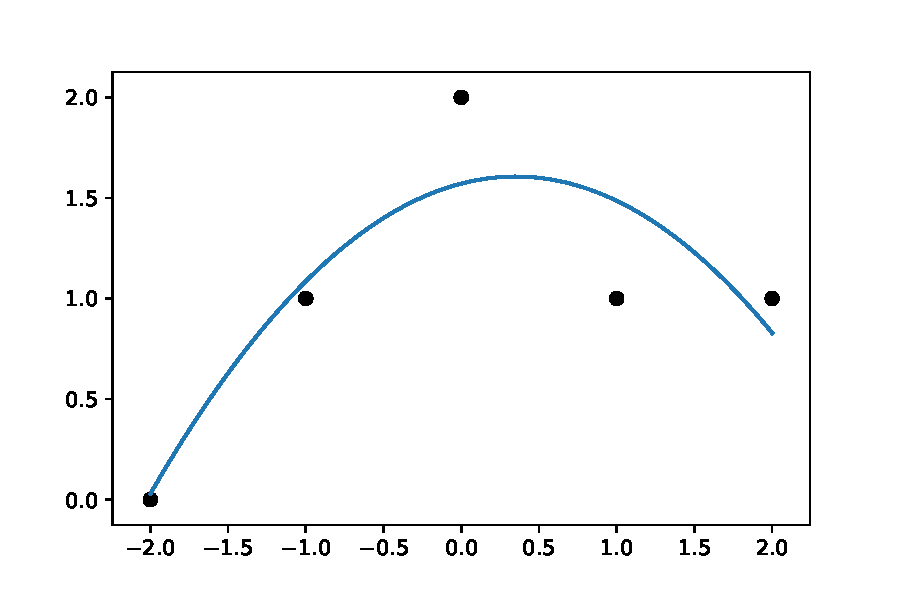
\includegraphics[width=\linewidth]{7-1.pdf}
\end{figure}

设置正则化参数分别为1和10,得到最小二乘解分别如下:
$$f(X)=1.53333333+0.18181818x-0.26666667x^2$$
$$f(X)=\frac{4}{3}+0.1x-\frac{1}{6}x^2$$

将上述三个函数绘图得:

\begin{figure}[H]
	\centering
	\caption{最小二乘及其正则化}
	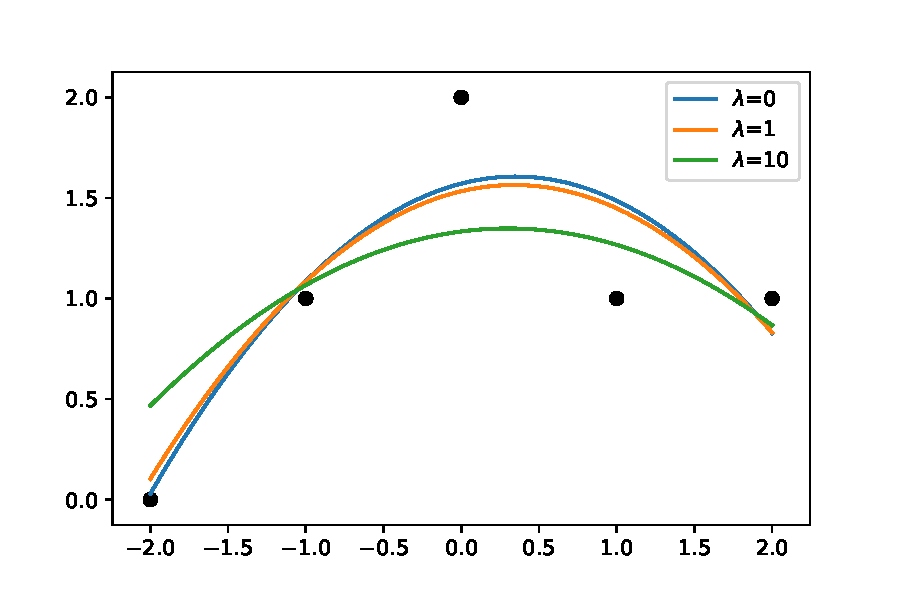
\includegraphics[width=\linewidth]{7-2.pdf}
\end{figure}

\paragraph{代码}

\begin{minted}{python}

lamda=0
I=np.eye(3)
I[0][0]=0
np.linalg.inv(np.matmul(X.T,X)+lamda*I)
theta=np.matmul(np.matmul(np.linalg.inv(np.matmul(X.T,X)+lamda*I),X.T),y)
x0=np.linspace(-2, 2, 100)
m0=len(x0)
x0=x0.reshape([100,1])
x0=np.concatenate((np.ones([100,1]),x0,x0**2), axis=1)
x0=x0.reshape([100,3])

plt.plot(np.linspace(-2, 2, 100),np.matmul(x0,theta),label='$\lambda$=0')
plt.scatter(x,y, color='black')
plt.savefig('7-1.pdf',dpi=200)
plt.show()

lamda=0
I=np.eye(3)
I[0][0]=0
np.linalg.inv(np.matmul(X.T,X)+lamda*I)
theta=np.matmul(np.matmul(np.linalg.inv(np.matmul(X.T,X)+lamda*I),X.T),y)
x0=np.linspace(-2, 2, 100)
m0=len(x0)
x0=x0.reshape([100,1])
x0=np.concatenate((np.ones([100,1]),x0,x0**2), axis=1)
x0=x0.reshape([100,3])
plt.plot(np.linspace(-2, 2, 100),np.matmul(x0,theta),label='$\lambda$=0')
print(theta)

lamda=1
I=np.eye(3)
I[0][0]=0
np.linalg.inv(np.matmul(X.T,X)+lamda*I)
theta=np.matmul(np.matmul(np.linalg.inv(np.matmul(X.T,X)+lamda*I),X.T),y)
x0=np.linspace(-2, 2, 100)
m0=len(x0)
x0=x0.reshape([100,1])
x0=np.concatenate((np.ones([100,1]),x0,x0**2), axis=1)
x0=x0.reshape([100,3])
plt.plot(np.linspace(-2, 2, 100),np.matmul(x0,theta),label='$\lambda$=1')
print(theta)

lamda=10
I=np.eye(3)
I[0][0]=0
theta=np.matmul(np.matmul(np.linalg.inv(np.matmul(X.T,X)+lamda*I),X.T),y)
x0=np.linspace(-2, 2, 100)
m0=len(x0)
x0=x0.reshape([100,1])
x0=np.concatenate((np.ones([100,1]),x0,x0**2), axis=1)
x0=x0.reshape([100,3])
plt.plot(np.linspace(-2, 2, 100),np.matmul(x0,theta),label='$\lambda$=10')
print(theta)



plt.scatter(x,y, color='black')
plt.legend()
plt.savefig('7-2.pdf',dpi=200)
plt.show()


\end{minted}

\section{第八章}


\subsection{题目1}
已知矩阵

$$
\mathbf{A} = 
\begin{gathered}
\begin{bmatrix} 
4 & -1 & 1\\
-1 & 3 & -2\\
1 & -2 & 3
\end{bmatrix}
\end{gathered}
$$

是一个对称矩阵,且其特征值为$\lambda_1=6,\lambda_2=3,\lambda_3=1$.
分别利用幂法、对称幂法、反幂法求其最大特征值和特征向量。
注意:可取初始向量$x^{(0)}=(111)^{T}.$

\paragraph{幂法}
假定$n\times n$的矩阵$\mathbf{A}$有$n$个特征值$\left|\lambda_1\right|> \left|\lambda_2\right| \geq \cdots \geq \left|\lambda_n\right|$, 对应线性无关的特征向量$\left\{\mathbf{v}^{\left(1\right)}, \mathbf{v}^{\left(2\right)},\cdots,\mathbf{v}^{\left(n\right)} \right\}$,

$\forall \mathbf{x} \in \mathbb{R}^n, \exists \beta_1,\beta_2,\cdots,\beta_n, st \ \mathbf{x} = \beta_1 \mathbf{v}^{\left(1\right)} + \beta_2 \mathbf{v}^{\left(2\right)} + \cdots + \beta_n \mathbf{v}^{\left(n\right)} = \sum_{j=1}^{n} \beta_j \mathbf{v}^{\left(j\right)}$

即
$$
\begin{aligned}
\mathbf{Ax} = &\sum_{j=1}^{n} \beta_j \mathbf{Av}^{\left(j\right)} = \sum_{j=1}^{n} \beta_j \lambda_j \mathbf{v}^{\left(j\right)} \\
\mathbf{A}^2\mathbf{x} = &\sum_{j=1}^{n} \beta_j \mathbf{Av}^{\left(j\right)} = \sum_{j=1}^{n} \beta_j \lambda_j^2 \mathbf{v}^{\left(j\right)} \\
\mathbf{A}^2\mathbf{x} = &\sum_{j=1}^{n} \beta_j \mathbf{Av}^{\left(j\right)} = \sum_{j=1}^{n} \beta_j \lambda_j^2 \mathbf{v}^{\left(j\right)} \\
&\vdots \\
\mathbf{A}^k\mathbf{x} =& \sum_{j=1}^{n} \beta_j \mathbf{Av}^{\left(j\right)} = \sum_{j=1}^{n} \beta_j \lambda_j^k \mathbf{v}^{\left(j\right)} \\
= &\lambda_1^k\left(\beta_1 \mathbf{v}^{\left(1\right)} + \sum_{j=2}^{n}\beta_j\left(\frac{\lambda_j}{\lambda_1}\right)^k\mathbf{v}^{\left(j\right)}\right)
\end{aligned}$$
由于
$\forall j \in \left\{2,\cdots,n\right\}, \left|\lambda_1\right| > \left|\lambda_j\right|$
,因此$\lim\limits_{k \to \infty}  \left(\frac{\lambda_j}{\lambda_1}\right)^k= 0$. 即
$$\lim\limits_{k \to \infty} \mathbf{A}^k \mathbf{x} = \lim\limits_{k \to \infty}\lambda_1^k \beta_1 \mathbf{v}^{\left(1\right)}$$
用$x_i^{\left(k\right)}$ 表示$\mathbf{x}^{\left(k\right)}$的第$i$个分量.由于
$$\frac{x_i^{\left(k+1\right)}}{x_i^{\left(k\right)}} \approx \frac{\lambda_1^{k+1} \beta_1 \mathbf{v}_i^{\left(1\right)}}{\lambda_1^k \beta_1 \mathbf{v}_i^{\left(k\right)}} = \lambda_1$$
需要注意, 当$\left|\lambda_1 \right| > 1$时, $\mathbf{x}^{\left(k\right)}$的各分量趋于无穷, 当$\left|\lambda_1\right| < 1$时, $\mathbf{x}^{\left(k\right)}$的各分量趋于0. 为了克服这一缺点, 需要将迭代向量规范化. 采用如下方式进行迭代:
$$
\left\{
\begin{aligned}
\mathbf{x}^{\left(0\right)} &= \mathbf{y}^{\left(0\right)} \neq \mathbf{0} \\
\mathbf{x}^{\left(k\right)} &= \mathbf{Ay}^{\left(k-1\right)} \\
\mathbf{y}^{\left(k\right)} & = \frac{\mathbf{x}^{\left(k\right)}}{\left|  \left|\mathbf{x}^{\left(k\right)} \right|\right|_{\infty}}
\end{aligned}
\right.$$

$$\lim\limits_{k \to \infty} \mathbf{y}^{\left(k\right)} = \frac{v^{\left(1\right)}}{\left|\left|\mathbf{v}^{\left(1\right)} \right| \right|}, \lim\limits_{k \to \infty} \left|\left|\mathbf{x} \right| \right|_{\infty } = \lambda_1$$.

易知最终的$\mathbf{x}$为所求特征向量.

\paragraph{结果}

解得最大特征值为$6.00000$,特征向量为$[1,-1,1]$,迭代次数为$22$次。

\paragraph{代码}

\begin{minted}{python}
def pow2(A, X, step, eps):
    l = 0
    cnt = 0
    err = 1
    while err > eps and cnt < step:
        cnt += 1
        Y = A * X
        C[cnt] = max(abs(Y))
        dc = abs(l - C[cnt])
        Y = (1 / C[cnt]) * Y
        dv = norm(X - Y)
        err = max(dc, dv)
        X = Y
        l = C[cnt]
    V = X
    return C, l, V
\end{minted}

\paragraph{对称幂法}
假设$\mathbf{A}$是对称矩阵, $\mathbf{A}$有$n$个实数特征向量$\left|\lambda_1 \right| > \left|\lambda_2 \right| > \cdots > \left|\lambda_n \right|$, 对应$n$个标准正交特征向量$\left\{\mathbf{v}^{\left(1\right)}, \mathbf{v}^{\left(2\right)}, \cdots, \mathbf{v}^{\left(n\right)} \right\}$. 

$\forall \mathbf{x}_0 \in \mathbb{R}^{n}, \mathbf{x}_0 = \beta_1 \mathbf{v}^{\left(1\right)} + \beta_2 \mathbf{v}^{\left(2\right)} + \cdots + \mathbf{v}^{\left(n\right)}$.

对于$\mathbf{x}_k = \mathbf{A}^k \mathbf{x}_0$,$\mathbf{x}_k = \beta_1 \lambda_1^k \mathbf{v}^{\left(1\right)} + \beta_2 \lambda_2^k \mathbf{v}^{\left(2\right)} + \cdots + \beta_n \lambda_n^k \mathbf{v}^{\left(n\right)}$.
因为$n$个特征向量标准正交, 因此
$$\mathbf{x}_k^T \mathbf{x}_k = \sum_{j=1}^{n} \beta_j^2 \lambda_j^{2k} = \beta_1^2 \lambda_1^{2k} \left[1 + \sum_{j=2}^{n}\left(\frac{\beta_j}{\beta_1}\right)^2 \left(\frac{\lambda_j}{\lambda_n} \right)^{2k} \right]$$
且
$$ \mathbf{x}_k^{T} \mathbf{A} \mathbf{x}_k = \sum_{j=1}^{n} \beta_j^2 \lambda_j^{2k+1} = \beta_1^2 \lambda_1^{2k+1} \left[ 1 + \sum_{j=2}^{n} \left(\frac{\beta_j}{\beta_1}\right)^2 \left(\frac{\lambda_j}{\lambda_1}\right)^{2k+1} \right] $$
于是
$$\lim\limits_{k \to \infty} \frac{\mathbf{x}_k^T \mathbf{A} \mathbf{x}_k}{\mathbf{x}_k^T \mathbf{x}_k} = \lambda_1, \lim\limits_{k \to \infty} \frac{\mathbf{x}_k}{\left|\left|\mathbf{x}_k \right|_{2} \right|} = \frac{\mathbf{v}^{\left(1\right)}}{\left|\left|\mathbf{v}^{\left(1\right)} \right| \right|_2}$$.

\paragraph{结果}

解得最大特征值为$6.00000$,特征向量为$[0.5774, -0.5773, 0.5773]$,迭代次数为$18$次。

\paragraph{代码}

\begin{minted}{python}
def sym_pow(A, X, step, eps):
    cnt = 0
    err = 1
    X = X / norm(X, 2)
    while err > eps and cnt < step:
        cnt += 1
        Y = A * X
        C[cnt] = X * Y
        dc = norm(Y, 2)
        err = norm(X - Y / norm(Y, 2), 2)
        X = Y / norm(Y, 2)
    V = X
    l = u
    return C, l, V
\end{minted}

\paragraph{反幂法}
设$\mathbf{A}$为$n\times n$阶非奇异矩阵, $\lambda$和$\mathbf{v}$为对应的特征向量, 即$\mathbf{Au} = \lambda \mathbf{v}$.

由于$\mathbf{A}^{-1}\mathbf{v} = \frac{1}{\lambda}\mathbf{v}$. 如果$\mathbf{A}$的特征值的顺序为$\left|\lambda_1\ \right| \geq \left|\lambda_2 \right| \geq \cdots \geq \left|\lambda_n \right|$,

则$\mathbf{A}^{-1}$的特征值$\left|\frac{1}{\lambda_n}  \right|\geq \left|\frac{1}{\lambda_{n-1}} \right| \geq \cdots \geq \left|\frac{1}{\lambda_1} \right|$.

因此, 若对矩阵$\mathbf{A}^{-1}$用幂法, 即可计算出$\mathbf{A}^{-1}$的最大特征值$\frac{1}{\lambda_n}$, 从而求得$\mathbf{A}$按模最小的特征值$\lambda_n$.

因为$\mathbf{A}^{-1}$的计算比较麻烦, 因此在实际运算时, 以求解方程组$\mathbf{Ax}^{\left(k+1 \right)} = \mathbf{x}^{\left(k\right)}$替代.

在本题中, 需要求解最大特征值. 根据圆盘定理, 矩阵$\textbf{A}$的特征值有上界$Ma$. 设$\lambda$为$\textbf{A}$的特征值, $k\in \mathbb{R}$. 则$\left(\mathbf{A}-k\mathbf{I}\right)\mathbf{x} = \left(\lambda - k\right) \mathbf{x}$. 此时令$k = Ma + 2$, 则$\left(\mathbf{A} - \left(Ma+2\right)\mathbf{I}\right)$的特征值均小于$0$. 设用反幂法求出$\left(\mathbf{A} - \left(Ma+2\right)\mathbf{I}\right)^{-1}$的绝对值最小特征值为$\left|\lambda^{*}\right|$, 则$\textbf{A}$的最大特征值为$Ma+2-\frac{1}{\left|\lambda^{*} \right|}$.

注: 圆盘定理:设$\mathbf{A}$是一个$n\times n$的矩阵, $\mathbb{R}_i$表示以$a_{ii}$为圆心, $\sum_{j=1,j\neq i}^{n}\left|a_{ij} \right|$的圆. 
令$$\mathbb{R}_i = \left\{z \in \mathbb{C}\bigg | \left|z-a_{ii} \right| \leq \sum_{j=1,j\neq i}^{n} \left|a_{ij} \right| \right\}$$
$\mathbf{A}$的特征值包含在$\bigcup_{i=1}^n \mathbb{R}_i $中.

\paragraph{结果}
~\\
\begin{enumerate}
	\item 当$\alpha = 5.5$时,特征值为$6.0000$,特征向量为$[-1, -1, -1]$,迭代次数为$10$次。
	\item 当$\alpha = 2.5$时,特征值为$3.0000$,特征向量为$[1,0.5,-0.5]$,迭代次数为$13$次。
	\item 当$\alpha = 0.6$时,特征值为$1.0000$,特征向量为$[0,1,1]$,迭代次数为$9$次。
\end{enumerate}

\paragraph{代码}

\begin{minted}{python}
def inv_pow(A, X, alpha, step, eps):
    n = A.size()
    A -= alpha * np.identity(n)
    l = 0
    cnt = 0
    err = 1
    while err > eps and cnt < step:
        cnt += 1
        Y = A / X
        C[cnt] = max(Y)
        dc = abs(l - C[cnt])
        Y = (1 / C[cnt]) * Y
        dv = norm(X - Y)
        err = max(dc, dv)
        X = Y
        l = C[cnt]
    l = alpha + 1 / C[cnt]
    V = X
    return C, l, V
\end{minted}



\subsection{题目2}

验证实验:写出PPT中关于Household变换示例中的$H_1,H_2,H_3$,并验证示例结果。


\paragraph{解答}

\newpage

\section{作业}


\subsection{1.1}

完成下列计算:
$\int_{0}^{1 / 4} e^{x^{2}} d x \approx \int_{0}^{1 / 4}\left(1+x^{2}+\frac{x^{2}}{2 !}+\frac{x^{6}}{3 !}\right) d x=\widehat{p}$
指出在这种情况下会出现哪种类型的误差,并将计算结果与真实值p=0.2553074606进行比较

\textbf{解答}

\begin{equation}
\begin{aligned} \int_{0}^{1 / 4} e^{x^{2}} d x & \approx \int_{0}^{1 / 4}\left(1+x^{2}+\frac{x^{4}}{3}+\frac{x^{6}}{3 !}\right) d x \\ &=\left(x+\frac{x^{3}}{3}+\frac{x^{5}}{5(2 !)}+\frac{x^{7}}{7(3 !)}\right)^{x=\frac{1}{4}}_{x=0}\\ &=\frac{1}{4}+\frac{1}{\sqrt{9}^{2}}+\frac{1}{10240}+\frac{x}{7(381)} \\ &=\frac{192807^{2}}{1146880} \approx 0.2553074428=\hat{p} \end{aligned}
\end{equation}



会出现截断误差,这导致了最后解的值小于真实值。

\subsection{1.2}

有时使用三角或代数恒等式,重新排列函数中的项,可以避免精度损失。求下列函数的等价公式,以避免精度损失。

1. $ln(x+1)-ln(x)$,其中x较大

2.$\sqrt{x^{2}+1}-x$,其中x较大

3.$\cos ^{2}(x)-\sin ^{2}(x)$,其中x约等于$\pi/4$

4.$\sqrt{\frac{1+\cos (x)}{2}}$,其中x约等于$\pi$



\textbf{解答}

1. 将原式$ln(x+1)-ln(x)$转换为$\ln \left(\frac{x+1}{x}\right)$

2.将原式$\sqrt{x^{2}+1}-x$转换为$\frac{1}{\sqrt{x^{2}+1+x}}$

3.将原式$\cos ^{2}(x)-\sin ^{2}(x)$转换为$\cos (2 x)$.

4.将原式$\sqrt{\frac{1+\cos (x)}{2}}$转换为$\cos (x / 2)$


\subsection{1.3}


讨论下列计算过程中的误差传播

(1)三个数的和:$$
p+q+r=\left(\widehat{p}+\epsilon_{p}\right)+\left(\widehat{q}+\epsilon_{q}\right)+\left(\widehat{r}+\epsilon_{r}\right)
$$

(2)两个数的商:$$\frac{p}{q}=\frac{\hat{p}+\epsilon_{p}}{\hat{q}+\epsilon_{q}}$$

(3)三个数的积:$$p q r=\left(\hat{p}+\epsilon_{p}\right)\left(\hat{q}+\epsilon_{q}\right)\left(\hat{r}+\epsilon_{r}\right)$$

\textbf{解答}

1.\begin{equation}\epsilon_{p}+\epsilon_{q}+\epsilon_{r}
\end{equation}
2.\begin{equation}
\frac{p}{q}=\frac{\hat{p}+\epsilon_{p}}{\hat{q}+\epsilon_{q}}=\frac{\hat{p}}{\hat{q}}+\frac{\epsilon_{p}+\frac{p}{\hat{q}} \epsilon_{q}}{\hat{q}+\epsilon_{q}}
\end{equation}


3.
\begin{equation}
\begin{aligned} p q r=&\left(\hat{p}+\epsilon_{p}\right)\left(\hat{q}+\epsilon_{q}\right)\left(\hat{r}+\epsilon_{r}\right) \\=& \hat{p} \hat{q} \hat{r}+\hat{p} \hat{r} \epsilon_{q}+\hat{q} \hat{r} \epsilon_{p}+\hat{p} \hat{q} \epsilon_{r}+\hat{r} \epsilon_{p} \epsilon_{q}+\hat{q} \epsilon_{p} \epsilon_{r}+\hat{p} \epsilon_{q} \epsilon_{r}+\epsilon_{p} \epsilon_{q} \epsilon_{r} \\=& \hat{p} \hat{q} \hat{r}+\left(\hat{p} \hat{r} \epsilon_{q}+\hat{q} \hat{r} \epsilon_{p}+\hat{p} \hat{q} \epsilon_{r}\right) \\ &+\left(\hat{r} \epsilon_{p} \epsilon_{q}+\hat{q} \epsilon_{p} \epsilon_{r}+\hat{p} \epsilon_{q} \epsilon_{r}\right)+\epsilon_{p} \epsilon_{q} \epsilon_{r} \end{aligned}
\end{equation}


\subsection{1.3}

设有泰勒展开式

$$\cos (h)=1-\frac{h^{2}}{2 !}+\frac{h^{4}}{4 !}+O\left(h^{6}\right)$$

和


$$\sin (h)=h-\frac{h^{3}}{3 !}+\frac{h^{5}}{5 !}+O\left(h^{7}\right)$$

判定它们和与积的近似阶:

\textbf{解答}

\begin{equation}
\begin{aligned} \cos (h)+\sin (h) &=1+h-\frac{h^{2}}{2}-\frac{h^{3}}{6}+\frac{h^{4}}{24}+\boldsymbol{O}\left(h^{5}\right) \\ \cos (h) \sin (h) &=h-\frac{2 h^{3}}{3}+\frac{2 h^{5}}{15}+\boldsymbol{O}\left(h^{7}\right) \end{aligned}
\end{equation}

\begin{equation}
\begin{array}{l}{\text { 中间的计算过程为}} \\ {\qquad\left(1+h+\frac{h^{2}}{2 !}+\frac{h^{3}}{3 !}+\frac{h^{4}}{4 !}\right)\left(h-\frac{h^{3}}{3 !}\right)=h+h^{2}+\frac{h^{3}}{3}-\frac{h^{5}}{24}-\frac{h^{6}}{36}-\frac{h^{7}}{144}}\end{array}
\end{equation}




\subsection{分析讨论题1}

求方程$x^2+(\alpha+\beta)x+10^9=0$的根,其中$\alpha=-10^9,\beta=-1$讨论如何设计计算格式才能有效地减少误差,提高计算精度。

\paragraph{分析}


设$a \neq 0, b^2 - 4ac > 0$,且有方程$ax^2 + bx + c = 0$,则通过如下二次根公式可解出方程的根:

\begin{equation}
x_1=\frac{-b+\sqrt{b^2-4ac}}{2a}  \quad \quad x_2=\frac{-b-\sqrt{b^2-4ac}}{2a}
\label{eq3}
\tag{1}
\end{equation}

通过将分子有理化,可以等价变换成下列公式

\begin{equation}
x_1=\frac{-2c}{b+\sqrt{b^2-4ac}} \quad \quad x_2=\frac{-2c}{b-\sqrt{b^2-4ac}}
\label{eq4}
\tag{2}
\end{equation}

\textbf{当$|b| \approx \sqrt{b^2 - 4ac}$,必须小心处理,以避免其值过小而引起巨量消失(catastrophic cancellation)而带来精度损失。}

\begin{itemize}
	\item 当$b > 0$的时候应使用公式(\ref{eq4})计算$x_1$,应使用公式(\ref{eq3})计算$x_2$。
	\item 当$b < 0$的时候应使用公式(\ref{eq3})计算$x_1$,应使用公式(\ref{eq4})计算$x_2$。
\end{itemize}



综上,应使用公式(\ref{eq3})计算$x_1$,应使用公式(\ref{eq4})计算$x_2$。



\subsection{分析讨论题2}

以计算$x^31$为例,讨论如何设计计算格式才能减少计算次数

\paragraph{解答}




\section{总结}

计算机科学根本上是一门抽象的科学,算法是其灵魂,数学是其基础,要求很高的实践性,而《数值计算》这门课几乎涵盖了计算机科学的这几大部分,既有适用于计算机求解的实用数值算法,又有严谨的数学推导与证明,还为许多高级算法、应用程序提供了基础设施的支持,有着很强的实践性,在许多任务中,这些基本的数值方法往往是效率的关键。

《数值计算》这门课在我的整个本科阶段的学习中也起到了承前启后的作用,既承接了之前的《高等数学》、《线性代数》等数学基础课程,又为后面更加高级的《算法分析》、《图形学》和《机器学习》等课程奠定了基础。在这门课中,我进一步体会到了数学与算法之美,能够更加注重自己抽象思维和计算思维的培养,更加注重算法功底的牢固,更加注重数学知识的深入与拓宽,更加注重实践,通过这几次实验,能够在实践中深化和检验理论。

感谢刘保东老师的辛勤付出!

\begin{thebibliography}{99}
	\bibitem{ref1} Mathews, John H., and Kurtis D. Fink. Numerical methods using MATLAB. Vol. 4. Upper Saddle River, NJ: Pearson Prentice Hall, 2004.
	\bibitem{ref3}Stefan Behnel, Robert Bradshaw, Craig Citro, Lisandro Dalcin, Dag Sverre Seljebotn and Kurt Smith. Cython: The Best of Both Worlds, Computing in Science and Engineering, 13, 31-39 (2011), DOI:10.1109/MCSE.2010.118
	\bibitem{ref4}Fernando Pérez and Brian E. Granger. IPython: A System for Interactive Scientific Computing, Computing in Science \& Engineering, 9, 21-29 (2007), DOI:10.1109/MCSE.2007.53
	\bibitem{ref5}Travis E, Oliphant. A guide to NumPy, USA: Trelgol Publishing, (2006).
	\bibitem{ref6}John D. Hunter. Matplotlib: A 2D Graphics Environment, Computing in Science \& Engineering, 9, 90-95 (2007), DOI:10.1109/MCSE.2007.55
	\bibitem{ref7}Jones E, Oliphant E, Peterson P, et al. SciPy: Open Source Scientific Tools for Python, 2001-, http://www.scipy.org/ [Online; accessed 2019-01-01].
	\bibitem{ref8}Wes McKinney. Data Structures for Statistical Computing in Python, Proceedings of the 9th Python in Science Conference, 51-56 (2010)
	\bibitem{ref9}Meurer A, Smith CP, Paprocki M, Čertík O, Kirpichev SB, Rocklin M, Kumar A, Ivanov S, Moore JK, Singh S, Rathnayake T, Vig S, Granger BE, Muller RP, Bonazzi F, Gupta H, Vats S, Johansson F, Pedregosa F, Curry MJ, Terrel AR, Roučka Š, Saboo A, Fernando I, Kulal S, Cimrman R, Scopatz A. SymPy: symbolic computing in Python, PeerJ Computer Science 3:e103 (2017)
\end{thebibliography}
\end{document}
